 \chapter{Results}\label{chap:Res}
\minitoc

In this chapter results of the W/Z cross section measurements at 2.76 TeV and their interpretation will be discussed. 
In Sec.~\ref{sec:flavCs} the cross sections measured for both lepton flavors are presented.
These results are used to test lepton universality in 2.76 TeV data.

Sec.~\ref{sec:CombCs} describes results obtained for combined W and Z cross sections. Additionally, in the subsection the cross section ratios are presented. In the final section, the interpretation of the results using the PDF profiling method is presented.

\section{Cross section measurement results}\label{sec:flavCs}

The cross sections are calculated separately for each boson and lepton flavor as described in Chap.~\ref{chap:Met}. The sources of uncertainties on the measurements are discussed in Chap.~\ref{chap:Unc}. The cross-sections have been measured in the fiducial region corresponding to the detector and selection criteria acceptance and extrapolated to the full phase space and new 13 TeV region, following the prescription from Chap.~\ref{chap:Met}. Tab.~\ref{tab:Wcs} summarizes the $W^{+/-}$ and Z cross sections obtained from 2.76 TeV data in all regions. 

The uncertainty coming from the luminosity measurement (labeled $lumi$) is a dominant. The data statistical uncertainty is labeled $stat.$ and is the second dominant uncertainty for the W and Z bosons cross section measurements. For W boson in the electron channel the systematic uncertainty is around 1\%, that makes it significantly lower, than the statistical uncertainty. For W boson cross section measurement in a muon channel the overall systematical uncertainty is higher because of the trigger scale factors, and is around 1.2\%. That makes it comparable with the statistical uncertainty.  

The obtained results are consistent between lepton flavors. 

%\begin{table}[!tbp]
\begin{center}
\caption{Number of observed candidates N and expected background events B, efficiency, acceptance and extrapolation correction factors for the W and Z bosons in electron and muon channels. Monte Carlo corrections are included in the $C_{W/Z}$ factors. The given uncertainties are the quadratic sum of statistical and systematic components.}
\label{tab:Values}
\begin{tabular}{l | c c c c }
\hline
\hline
 & $N_{W/Z}^{sig}$ & $C_{W/Z}$ & $A_{W/Z}$ & $E_{W/Z}$ \\
 \hline
& \multicolumn{4}{c}{Electron channel}\\
 \hline
 $W^{+}\to e\nu$  & & & & \\
 $W^{-}\to e\nu$ & & & & \\
 $Z \to ee$ & & & & \\
 \hline
 & \multicolumn{4}{c}{Muon channel} \\
  \hline
  $W^{+}\to \mu\nu$  & & & & \\
 $W^{-}\to \mu\nu$ & & & & \\
 $Z \to \mu \mu $ & & & & \\
 \hline
\end{tabular}
\end{center}
\end{table}

\begin{table}[!tb]
\caption{Results on a fiducial $\sigma^{fid}$ and total cross-section measurement for $W^{+}$, $W^{-}$ and Z bosons in electron and muon channels. The cross-sections are shown with their statistical, systematical and luminosity uncertainties (and extrapolation error for total cross-section) quoted in that order}
\label{tab:Wcs}
\begin{center}
\begin{tabular}{| l | c | c |}
\hline
 & value $\pm$ stat $\pm$ syst $\pm$ lumi ($\pm$ ext)& value $\pm$ stat $\pm$ syst $\pm$ lumi ($\pm$ ext) \\
 \hline
 \hline
 & \multicolumn{2}{c|}{W in electron channel}\\
& $W^{+}\to e\nu$ & $W^{-}\to e\nu$ \\

\hline
$\sigma^{fid}_{W}$ [pb]  & \sigfidWplusenunolabel & \sigfidWminenunolabel \\
$\sigma^{tot}_{W}$ [pb] & \sigtotWplusenunolabel & \sigtotWminenunolabel \\
$\sigma^{13}_{W}$ [pb] & \sigTrWplusenunolabel & \sigTrWminenunolabel \\
\hline
\hline
 & \multicolumn{2}{c|}{W in muon channel}\\
& $W^{+}\to \mu\nu$ & $W^{-}\to \mu\nu$\\
\hline
$\sigma^{fid}_{W}$ [pb] & \sigfidWplusmununolabel & \sigfidWminmununolabel \\
$\sigma^{tot}_{W}$ [pb]  & \sigtotWplusmununolabel & \sigtotWminmununolabel \\
$\sigma^{13}_{W}$ [pb]  & \sigTrWplusmununolabel & \sigTrWminmununolabel \\
\hline
%\hline
 %& \multicolumn{2}{c|}{$W^{+-}$ } \\
%& $W \to e\nu$ & $W \to \mu \nu$ \\
%\hline
%$\sigma^{fid}_{W}$ &  & \\
%$\sigma^{tot}_{W}$ & & \\
%$\sigma^{13}_{W}$ & & \\
%\hline
\hline
 & \multicolumn{2}{c|}{Z} \\
& $Z \to ee$ & $ Z \to \mu\mu$ \\
\hline
$\sigma^{fid}_{Z}$  [pb] &\sigfidZeenolabel &  \sigfidZmumunolabel \\
$\sigma^{tot}_{Z}$  [pb] & \sigtotZeenolabel & \sigtotZmumunolabel \\
$\sigma^{13}_{Z}$ [pb]  & \sigTrZeenolabel & \sigTrZmumunolabel \\
\hline
\end{tabular}
\end{center}
\end{table}

\subsection{Lepton universality test}\label{sec:LeptUnivers}

\begin{figure}[!tb]
\begin{center}
\begin{minipage}[h]{0.8\linewidth}
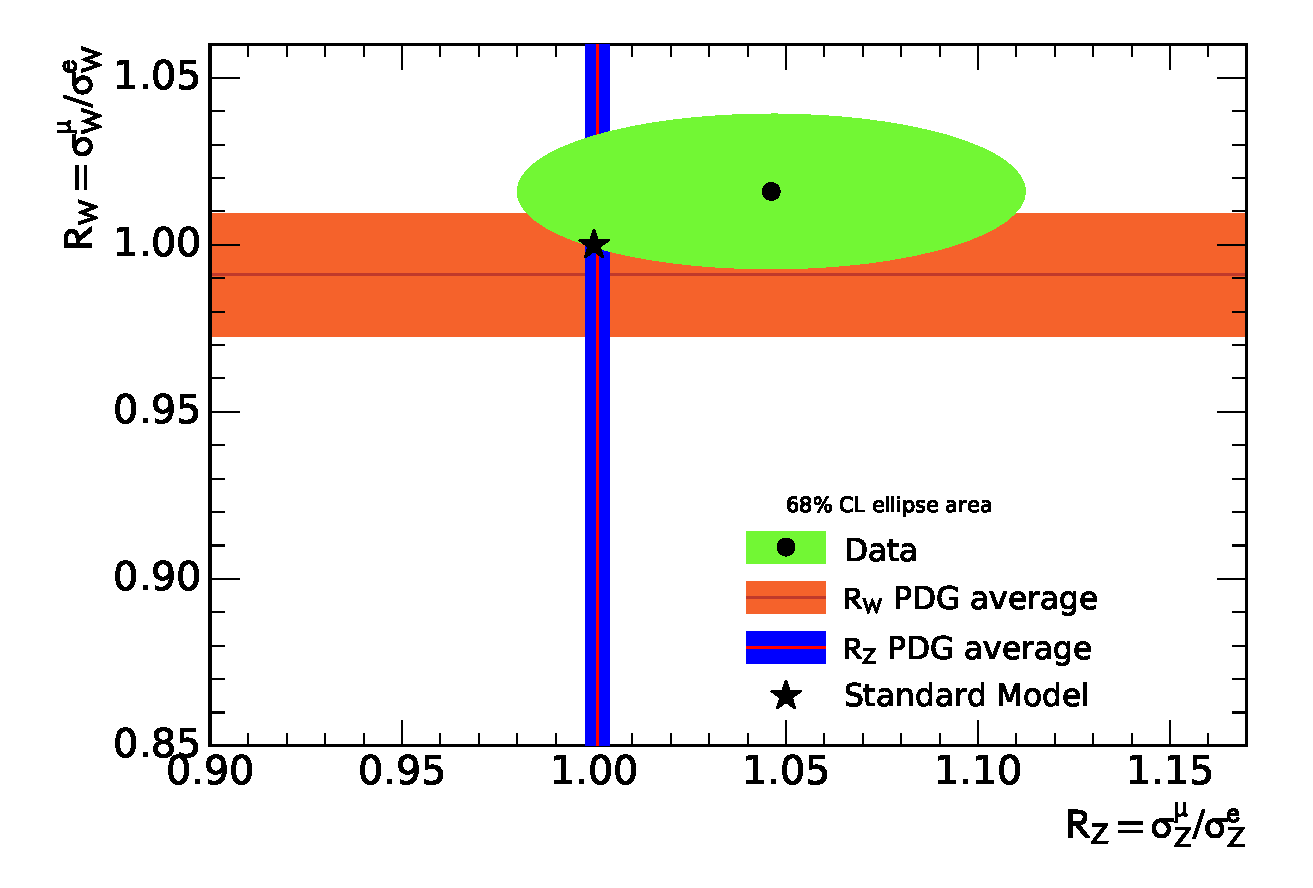
\includegraphics[width=1\textwidth]{Results/Univers.pdf}
\end{minipage}
\caption{The correlated measurement of the muon-to-electron fiducial cross section ratios in the W and the Z channels. The vertical (horizontal) band represents the uncertainty of the corresponding Z (W) branching fractions based on the current world average data. The green ellipse illustrates the 68\% CL for the correlated measurement of $R_W$ and $R_Z$.}
\label{fig:LeptUnivers}
\end{center}
\end{figure}


Because of the lepton universality of the Standard Model (SM), the results, obtained in electron and muon channels are expected to agree with each other. The $W^{\pm}$ cross sections are calculated in fiducial region following the prescription from Sec.~\ref{sec:Wcs}:
\begin{center}
$\sigma^{fid}_{W}(\wenu) = \valWenu  \pm \statWenu (stat.) \pm \sysWenu (sys.) \pm \lumiWenu (lumi.) \, [pb]$,\\
$\sigma^{fid}_{W}(\wmunu) = \valWmunu  \pm \statWmunu (stat.) \pm \sysWmunu (sys.) \pm \lumiWmunu (lumi.) \, [pb]$,
\end{center} 
which gives a ratio:
\begin{center}
$R_{W}=\frac{\sigma^{\mu}_W}{\sigma^{e}_W} = \frac{BR(\wmunu)}{BR(\wenu)}= \valWunivers \pm \sysWunivers (sys.) \pm \statWunivers (stat.)$,
\end{center}
that is in agreement within the uncertainty with the SM prediction and the world average of this value  $R^{world}_W=0.991\pm0.018$ \cite{Agashe:2014kda}. 

Similarly, such ratio can be measured in a Z boson decays as:
\begin{center}
$R_{Z}=\frac{\sigma^{\mu}_Z}{\sigma^{e}_Z} = \frac{BR(Z\to \mu\mu)}{BR(Z \to ee)}= \valZunivers \pm \sysZunivers(sys.) \pm \statZunivers (stat.)$.
\end{center}
This ratio value uncertainty is dominated by the statistical error. The world average for this ratio value is $R^{world}_Z=1.0009 \pm 0.0028$ \cite{Agashe:2014kda}. 

The comparison of $R_W$ and $R_Z$ taking into account the correlated systematic uncertainties with the respect of world average is shown in Fig.~\ref{fig:LeptUnivers}. The correlation matrix for $R_W$ and $R_Z$ can be found in Appendix~\ref{app:Cor}. The ellipse angle is obtained from the correlation matrix using the eigenvector decomposition and corresponds to the angle between x axis and the one of the 2 eigenvectors. The obtained values agree, within the 68\% confidence level, with the Standard Model expectations and the world averages.




\section{Combined results}\label{sec:CombCs}

Since the results for different analysis are agree withing the uncertainty, it is possible to perform averaging as described in Sec.~\ref{sec:Aver}. The combination is done in the fiducial region, and then combined cross sections are extrapolated to the full and new 13 TeV regions. The systematic uncertainties used in the averaging procedure are taken from Chap.~\ref{chap:Unc}, taking into account correlations between them. The common luminosity uncertainty is excluded from the combination process.

\begin{table}[!tb]
\caption{Results on a fiducial $\sigma^{fid}$ and total cross-section measurement for $W^{+}$, $W^{-}$ and Z bosons in electron and muon channels. The cross-sections are shown with their statistical, systematical and luminosity uncertainties (and extrapolation error for total cross-section) quoted in that order}
\label{tab:csComb}
\begin{center}
\begin{tabular}{| l | c | c |}
\hline
 & value $\pm$ stat $\pm$ syst $\pm$ lumi ($\pm$ ext)& value $\pm$ stat $\pm$ syst $\pm$ lumi ($\pm$ ext) \\
 \hline
 \hline
 & \multicolumn{2}{c|}{$W^{+/-}$}\\
& $W^{+}\to l\nu$ & $W^{-}\to l\nu$ \\

\hline
$\sigma^{fid}_{W}$ [pb]  & $\valfidWp \pm \statfidWp \pm \sysfidWp \pm \lumifidWp$ & $\valfidWm \pm \statfidWm \pm \sysfidWm \pm \lumifidWm$ \\
$\sigma^{tot}_{W}$ [pb] & $\valfullWp \pm \statfullWp \pm \sysfullWp \pm \lumifullWp \pm \extrfullWp$ & $\valfullWm \pm \statfullWm \pm \sysfullWm \pm \lumifullWm \pm \extrfullWm$ \\
$\sigma^{13}_{W}$ [pb] & $\valthrWp \pm \statthrWp \pm \systhrWp \pm \lumithrWp$ & $\valthrWm \pm \statthrWm \pm \systhrWm \pm \lumithrWm$ \\
\hline
\hline
& \multicolumn{2}{c|}{$W \to l \nu$} \\
\hline
$\sigma^{fid}_{W}$ [pb] & \multicolumn{2}{c|}{$\valfidWtot \pm \statfidWtot \pm \sysfidWtot \pm \lumifidWtot$} \\
$\sigma^{tot}_{W}$ [pb]  & \multicolumn{2}{c|}{$\valfullWtot \pm \statfullWtot \pm \sysfullWtot \pm \lumifullWtot \pm \extrfullWtot$} \\
$\sigma^{13}_{W}$ [pb]  & \multicolumn{2}{c|}{$\valthrWtot \pm \statthrWtot \pm \systhrWtot \pm \lumithrWtot$} \\
\hline
%\hline
 %& \multicolumn{2}{c|}{$W^{+-}$ } \\
%& $W \to e\nu$ & $W \to \mu \nu$ \\
%\hline
%$\sigma^{fid}_{W}$ &  & \\
%$\sigma^{tot}_{W}$ & & \\
%$\sigma^{13}_{W}$ & & \\
%\hline
\hline
 & \multicolumn{2}{c|}{$Z \to ll$} \\
\hline
$\sigma^{fid}_{Z}$ [pb] & \multicolumn{2}{c|}{$\valfidZ \pm \statfidZ \pm \sysfidZ \pm \lumifidZ$} \\
$\sigma^{tot}_{Z}$ [pb]  & \multicolumn{2}{c|}{$\valfullZ \pm \statfullZ \pm \sysfullZ \pm \lumifullZ \pm \extrfullZ$} \\
$\sigma^{13}_{Z}$ [pb]  & \multicolumn{2}{c|}{$\valthrZ \pm \statthrZ \pm \systhrZ \pm \lumithrZ$} \\
\hline
\end{tabular}
\end{center}
\end{table}

The resulting cross sections are summarized in Tab.~\ref{tab:csComb}.  The combination procedure allows to significantly reduce statistical uncertainty of the measurement compared to the separate cross sections. The systematic uncertainty is also visibly reduced, because most of the sources are uncorrelated for different flavors of the analysis. The combination yields good $\chi^2/NDF\, \approx$ 1/3 indicating a good agreement between measurements.  The W cross section is calculated from the combined $W^+$ and $W^-$ cross sections and is also in a good agreement with separate channels (Fig.~\ref{fig:Z} b).

The theoretical predictions are obtained at NLO and NNLO level of precision.  The NLO calculations are performed using the MCFM generator\cite{MCFM}, interfaced for a faster calculation with APPLGRID\cite{APPLGRID}, that provides an $x$ vs $Q^2$ grid for a calculation and convolution with a given PDF set. The NNLO predictions have been provided from the FEWZ  program \cite{FEWZ}.

\begin{figure}[!tbp]
\begin{minipage}[h]{0.45\linewidth}
\center{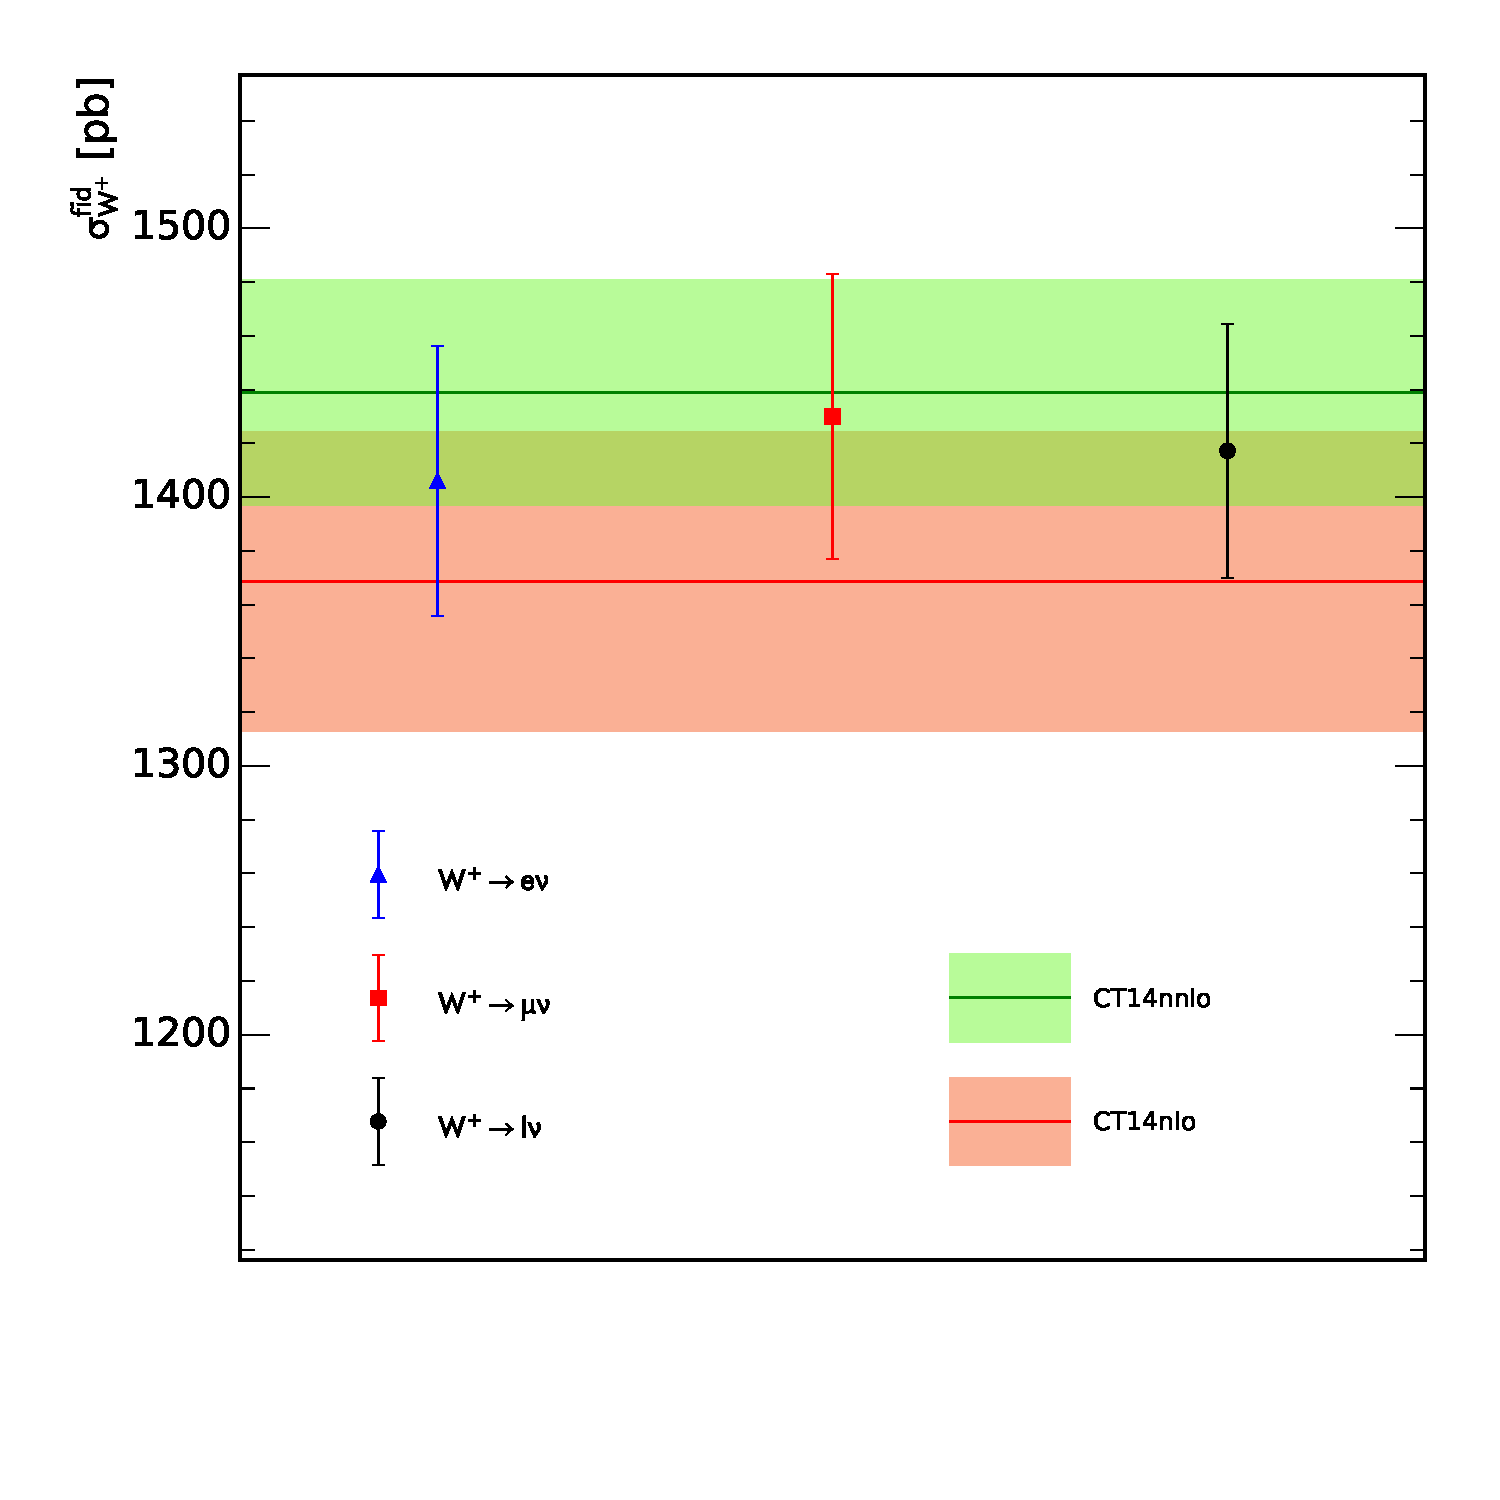
\includegraphics[width=1\textwidth]{Results/NNLOCompWPlus.pdf} \\ a)}
\end{minipage}
\hfill
\begin{minipage}[h]{0.45\linewidth}
\center{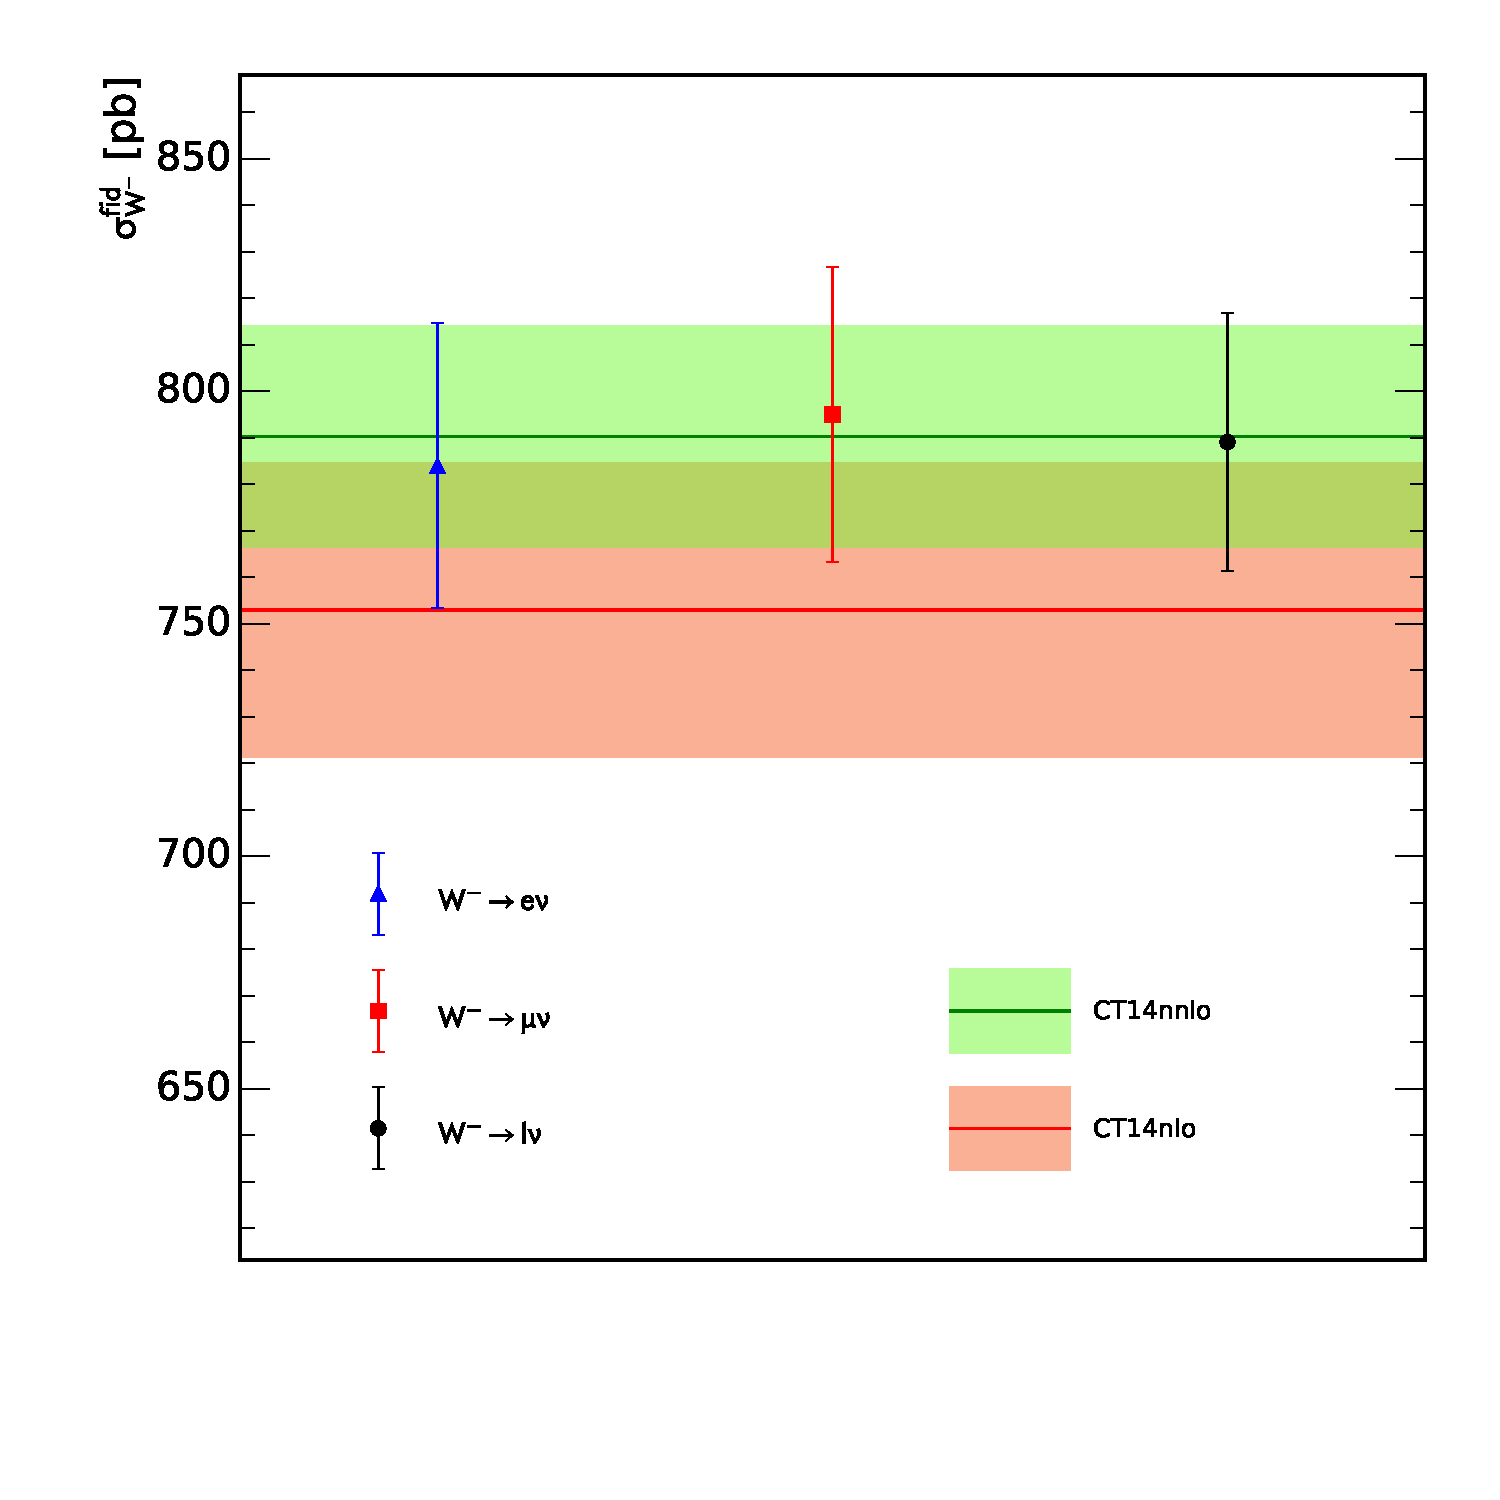
\includegraphics[width=1\textwidth]{Results/NNLOCompWMinus.pdf}\\ b)}
\end{minipage}
\caption{The NLO and NNLO theoretical predictions calculated using the CT14nnlo PDF set compared to the measured fiducial cross sections as given in Tab.~\ref{tab:Wcs} and Tab.~\ref{tab:csComb} for a) $\sigma^{fid}_{W^{+}}$ and b) $\sigma^{fid}_{W^-}$. The blue and red dots correspond to the electron and muon channels respectively, while black dots  represent the combined channel. The NLO and NNLO predictions are presented by the red and green lines with error-bands respectively. }
\label{fig:WpNNLO}
\end{figure}

\begin{figure}[!tbp]
\begin{minipage}[h]{0.45\linewidth}
\center{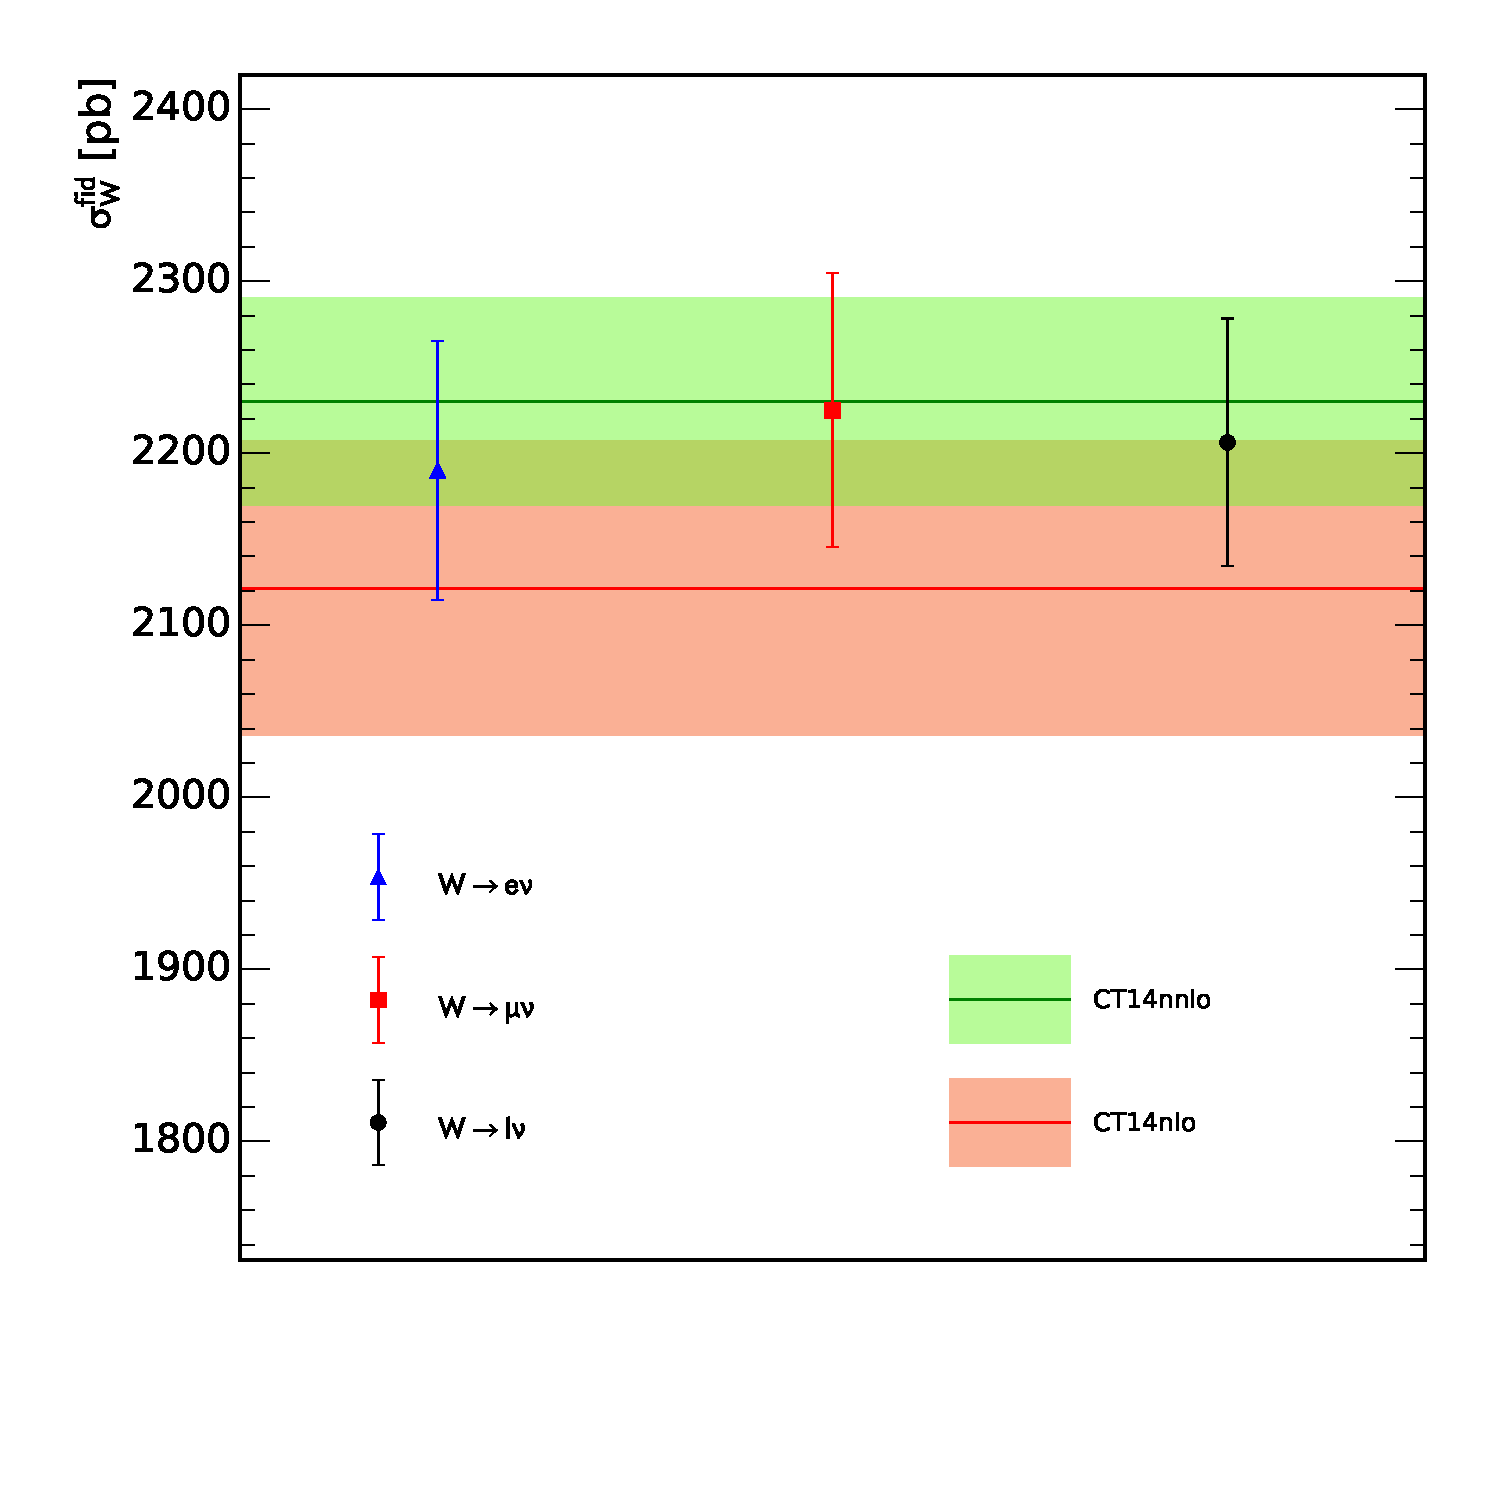
\includegraphics[width=1\textwidth]{Results/NNLOCompW.pdf} \\ a)}
\end{minipage}
\hfill
\begin{minipage}[h]{0.45\linewidth}
\center{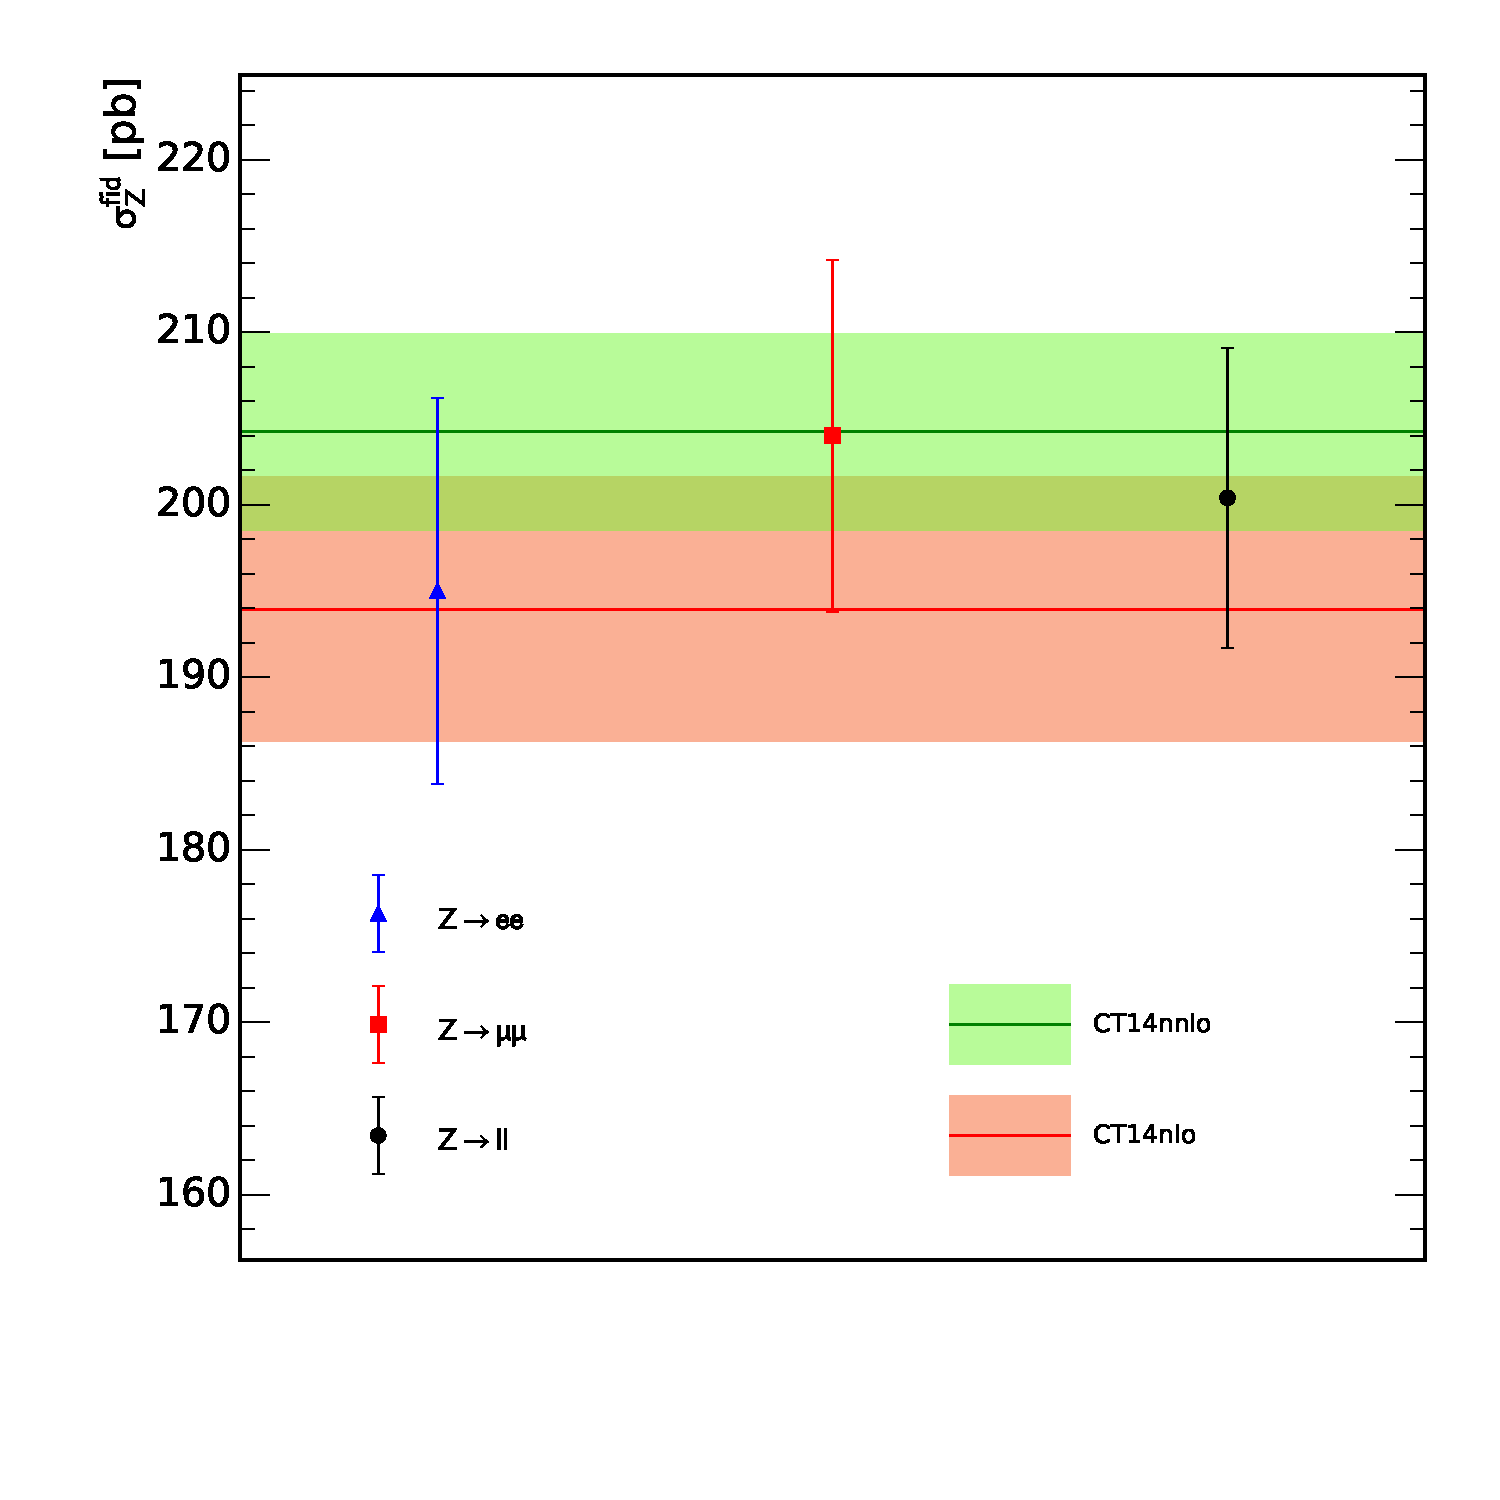
\includegraphics[width=1\textwidth]{Results/NNLOCompZ.pdf} \\ b)}
\end{minipage}
\caption{The NLO and NNLO theoretical predictions calculated using the CT14nnlo PDF set compared to the measured fiducial cross sections as given in Tab.~\ref{tab:Wcs} and Tab.~\ref{tab:csComb} for a) $\sigma^{fid}_W$ and b) $\sigma^{fid}_Z$. he blue and red dots correspond to the electron and muon channels respectively, while black dots  represent the combined channel. The NLO and NNLO predictions are presented by the red and green lines with error-bands respectively.}
\label{fig:Z}
\end{figure}

The comparison of NLO and NNLO predictions for CT14nnlo\cite{CT14} PDF set for the cross sections in the fiducial region with the experimental data for $W^{+}$, $W^{-}$, $W^{\pm}$  and $Z$ in electron, muon and combined channels are shown in Fig.~\ref{fig:WpNNLO} and Fig.~\ref{fig:Z}. The NLO and NNLO cross sections agree with each other and with experimental data withing the PDF uncertainty. The values of NLO cross section predictions are smaller, than the obtained experimental results and have a higher uncertainty. The NNLO predictions have better agreement and a similar uncertainty.

\begin{figure}[!tbp]
\begin{center}
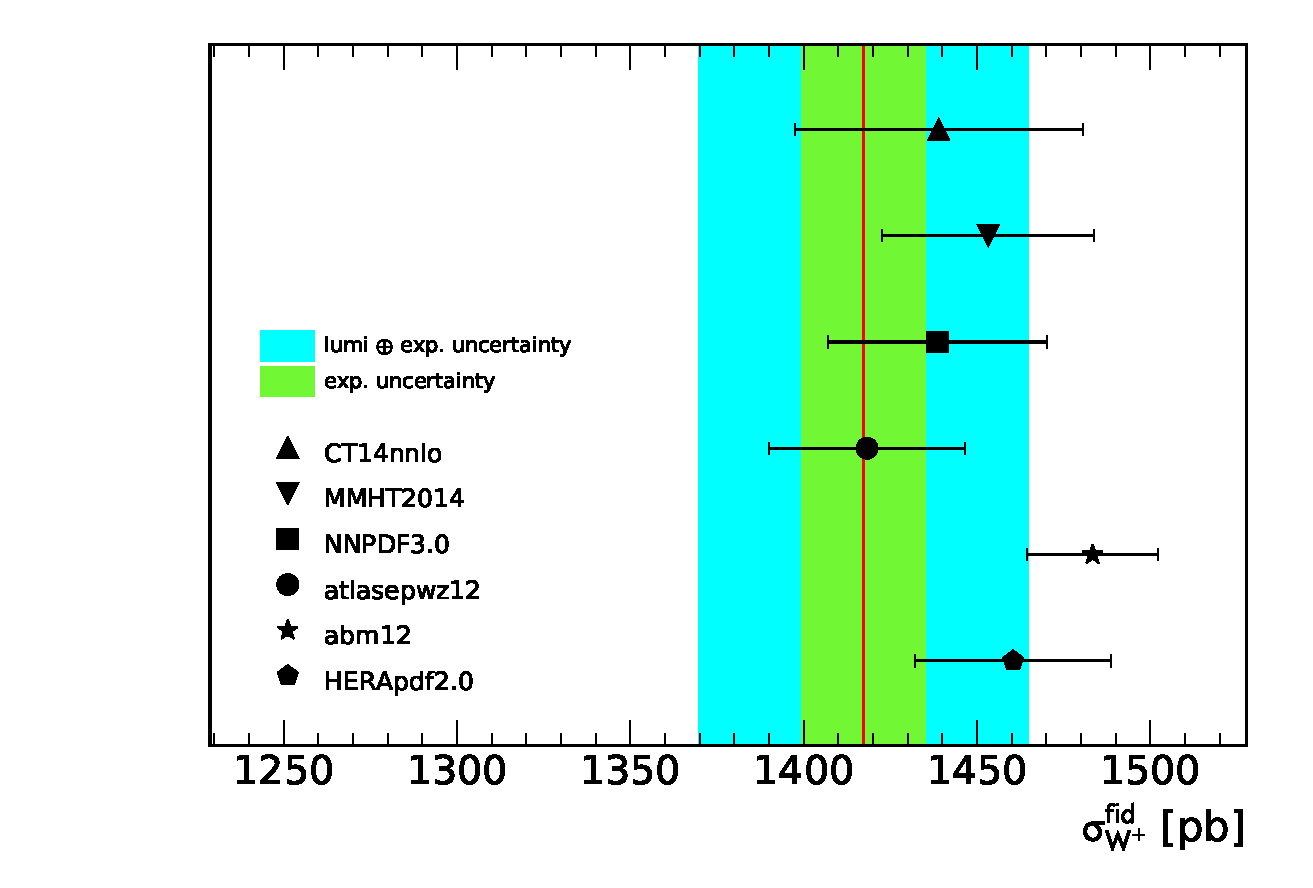
\includegraphics[width=0.65\textwidth]{Results/NNLOWPlus.pdf}
\end{center}
\caption{ NNLO predictions for the fiducial cross section $\sigma^{fid}_{W^{+}}$ in pb for the six PDFs CT14nnlo, MMHT2014, NNPDF3.0, ATLASepWZ12, abm12, HERApdf2.0 compared to the measured fiducial cross section as given in Tab.~\ref{tab:csComb}. The green (cyan) band corresponds to the experimental uncertainty without (with) the luminosity uncertainty. The theory predictions are given with the corresponding PDF uncertainties shown as error bands. }
\label{fig:NNLODifPDFWP}
\end{figure}

\begin{figure}[!tbp]
\begin{center}
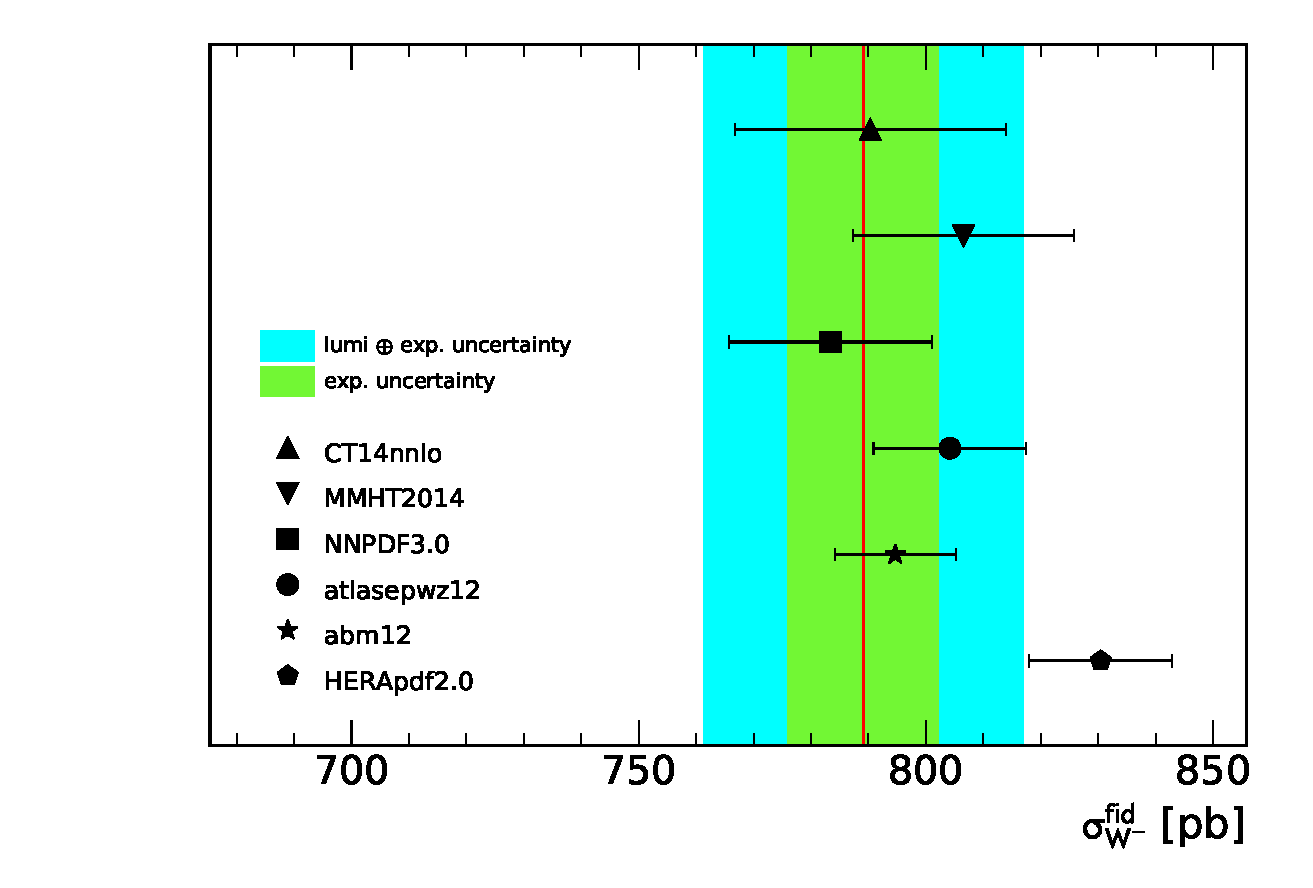
\includegraphics[width=0.65\textwidth]{Results/NNLOWMinus.pdf}
\end{center}
\caption{NNLO predictions for the fiducial cross section $\sigma^{fid}_{W^{-}}$ in pb for the six PDFs CT14nnlo, MMHT2014, NNPDF3.0, ATLASepWZ12, abm12, HERApdf2.0 compared to the measured fiducial cross section as given in Tab.~\ref{tab:csComb}. The green (cyan) band corresponds to the experimental uncertainty without (with) the luminosity uncertainty. The theory predictions are given with the corresponding PDF uncertainties shown as error bands.}
\label{fig:NNLODifPDFWm}
\end{figure}

\begin{figure}[!tbp]
\begin{center}
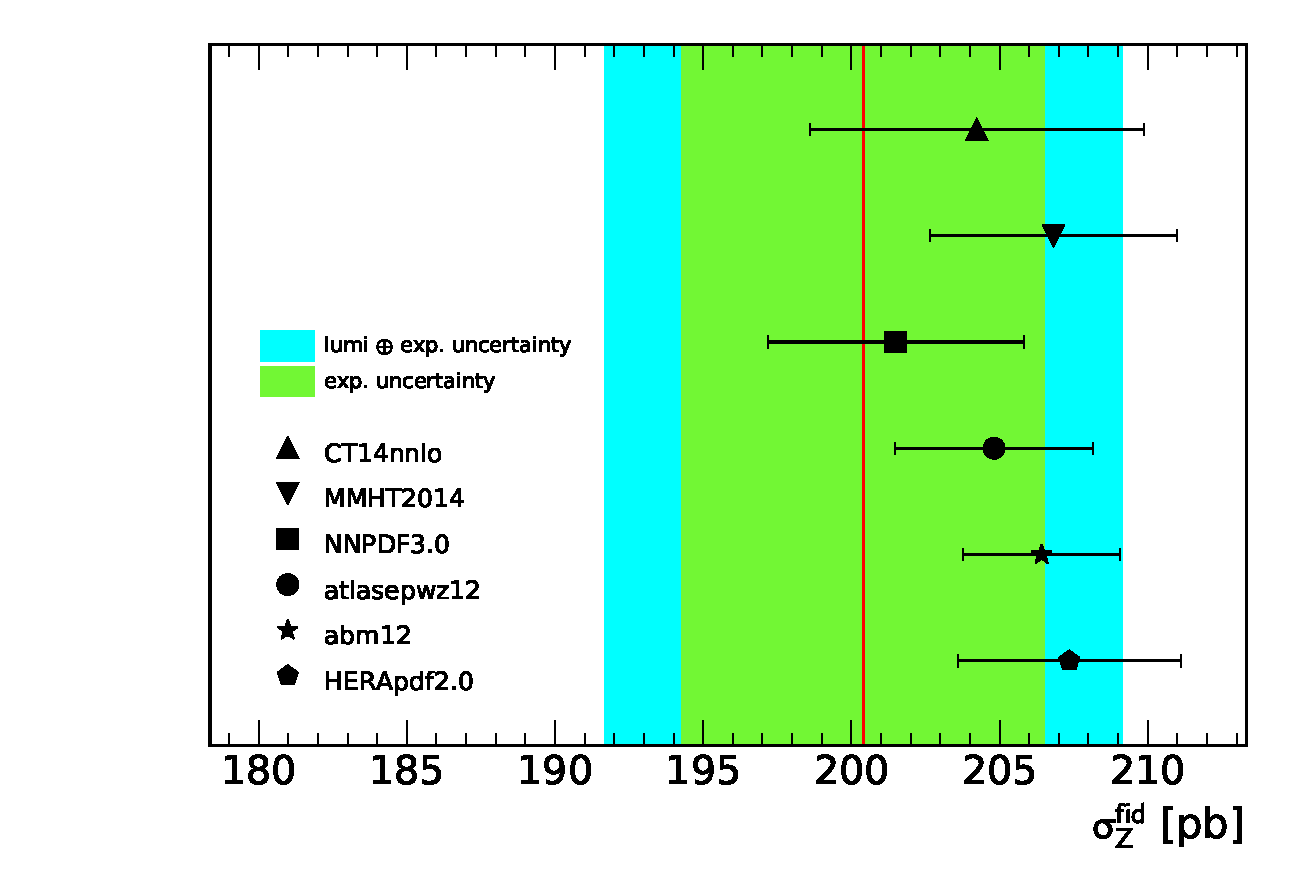
\includegraphics[width=0.65\textwidth]{Results/NNLOZ.pdf}
\end{center}
\caption{Predictions for the fiducial cross section $\sigma^{fid}_Z$ in pb for the six PDFs CT14nnlo, MMHT2014, NNPDF3.0, ATLASepWZ12, abm12, HERApdf2.0 compared to the measured fiducial cross section as given in Tab.~\ref{tab:csComb}. The green (cyan) band corresponds to the experimental uncertainty without (with) the luminosity uncertainty. The theory predictions are given with the corresponding PDF uncertainties shown as error bands.}
\label{fig:NNLODifPDFZ}
\end{figure}

Additionally, the obtained $W^+$, $W^-$ and $Z$ cross sections in a combined channel are compared to the NNLO predictions for a following PDF sets: ABM12nlo\cite{ABM12}, CT14nnlo\cite{CT14}, MMHTnnlo\cite{MMHT}, ATLASepWZ12\cite{ATLASEP}, NNPDF3.0\cite{NNPDF23} and HERApdf2.0nnlo\cite{HERAPDF} in Fig.~\ref{fig:NNLODifPDFWP}-\ref{fig:NNLODifPDFZ}. The best overall agreement is achieved in a NNPDF3.0 pdf set.  Additional NNLO comparisons for full and 13 TeV regions could be found in the Appendix~\ref{app:NLO}.  

Fig ~\ref{fig:ZcsResults} shows the LH, Tevatron and other pp and p$\bar{p}$ results on measuring W and Z-boson cross sections. It is the same plot that has shown earlier in Chap.~\ref{chap:Theory} (Fig.~\ref{fig:Zcs}), however the cross sections measured in this analysis are added. The cross sections measured at $\sqrt{s}$ = 2.76 TeV are fully consistent with earlier LHC results and CT14 NNLO theoretical predictions. The good overall agreement is achieved on the whole center-of-mass energies range accessible at LHC.


\begin{figure}[!h]
\begin{minipage}[h]{1.0\linewidth}
\center{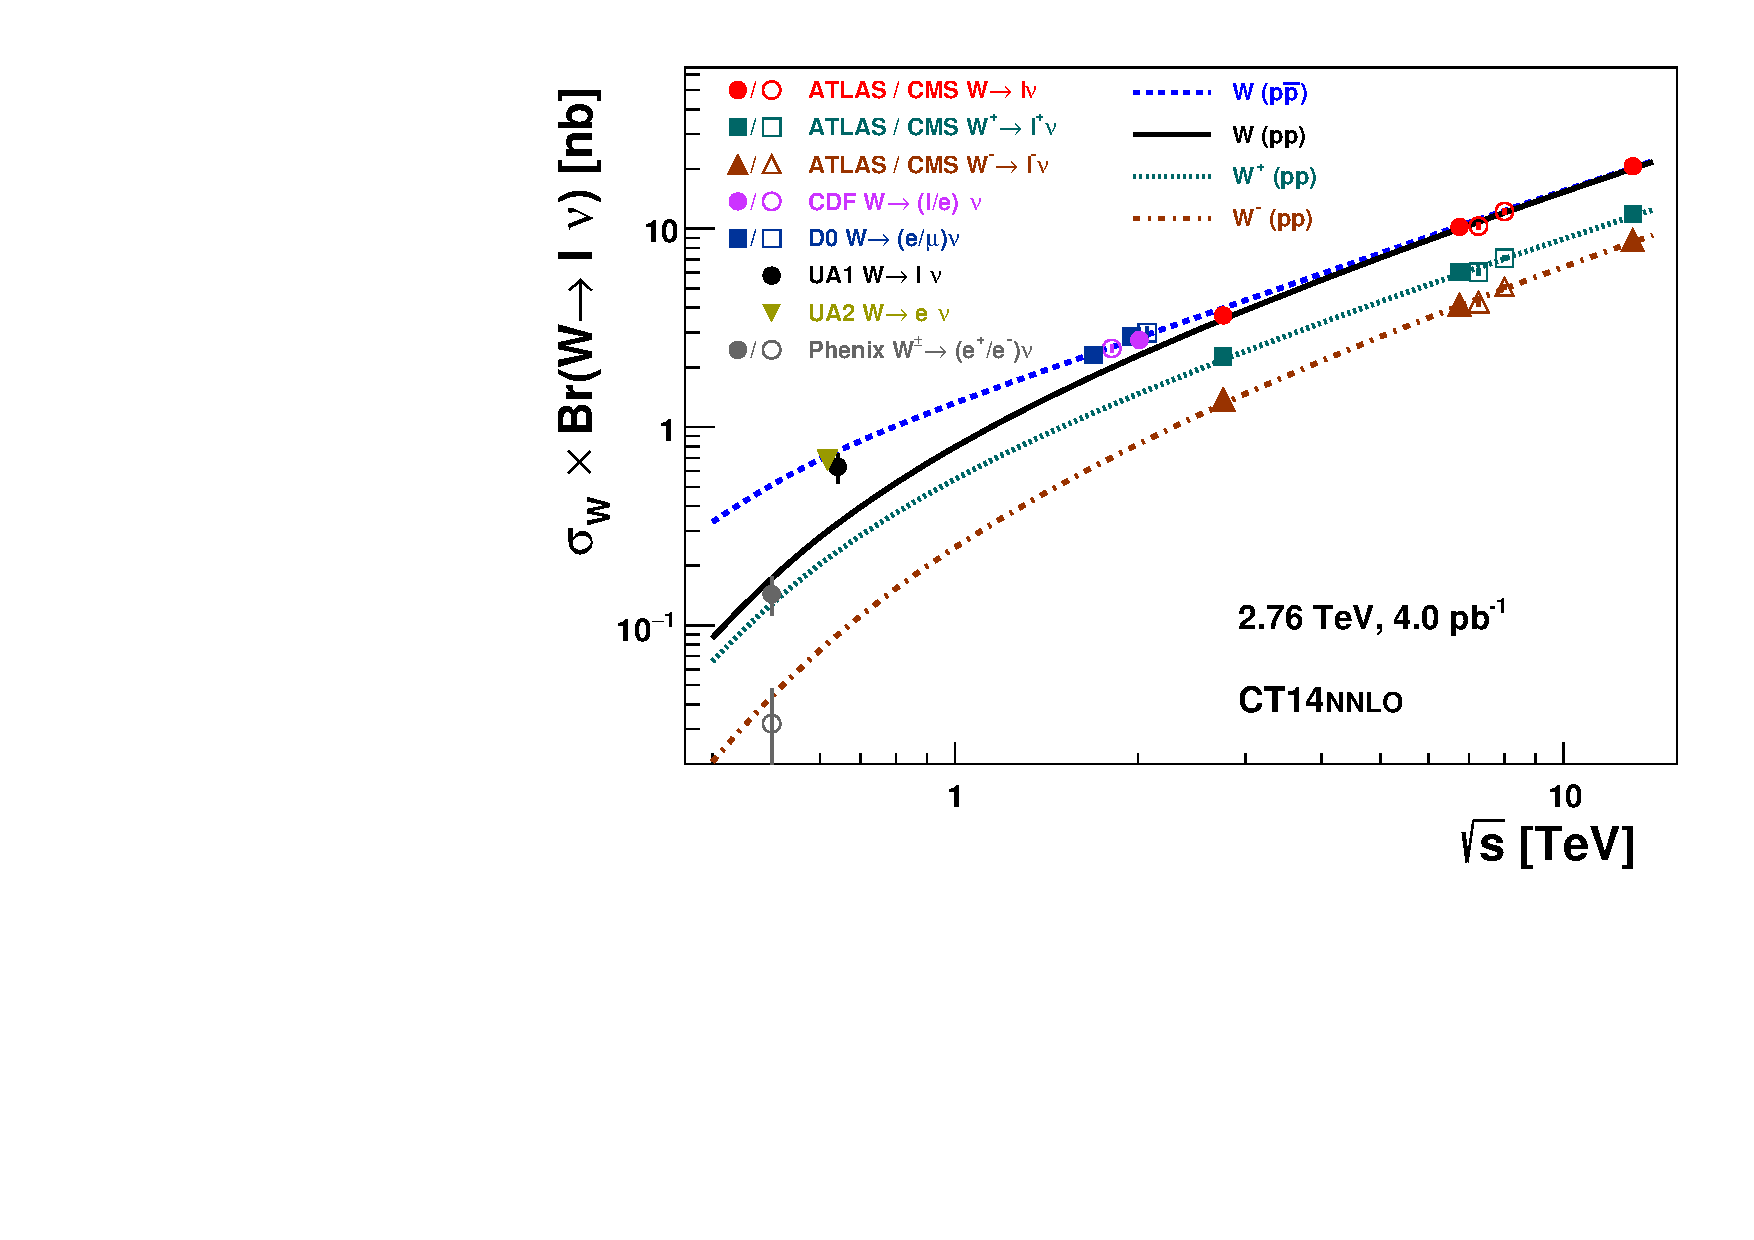
\includegraphics[width=0.7\linewidth]{Results/SigmaWatNNLOCombwithCMSLogx.pdf} \\ a)}
\end{minipage}
\vfill
\begin{minipage}[h]{1.0\linewidth}
\center{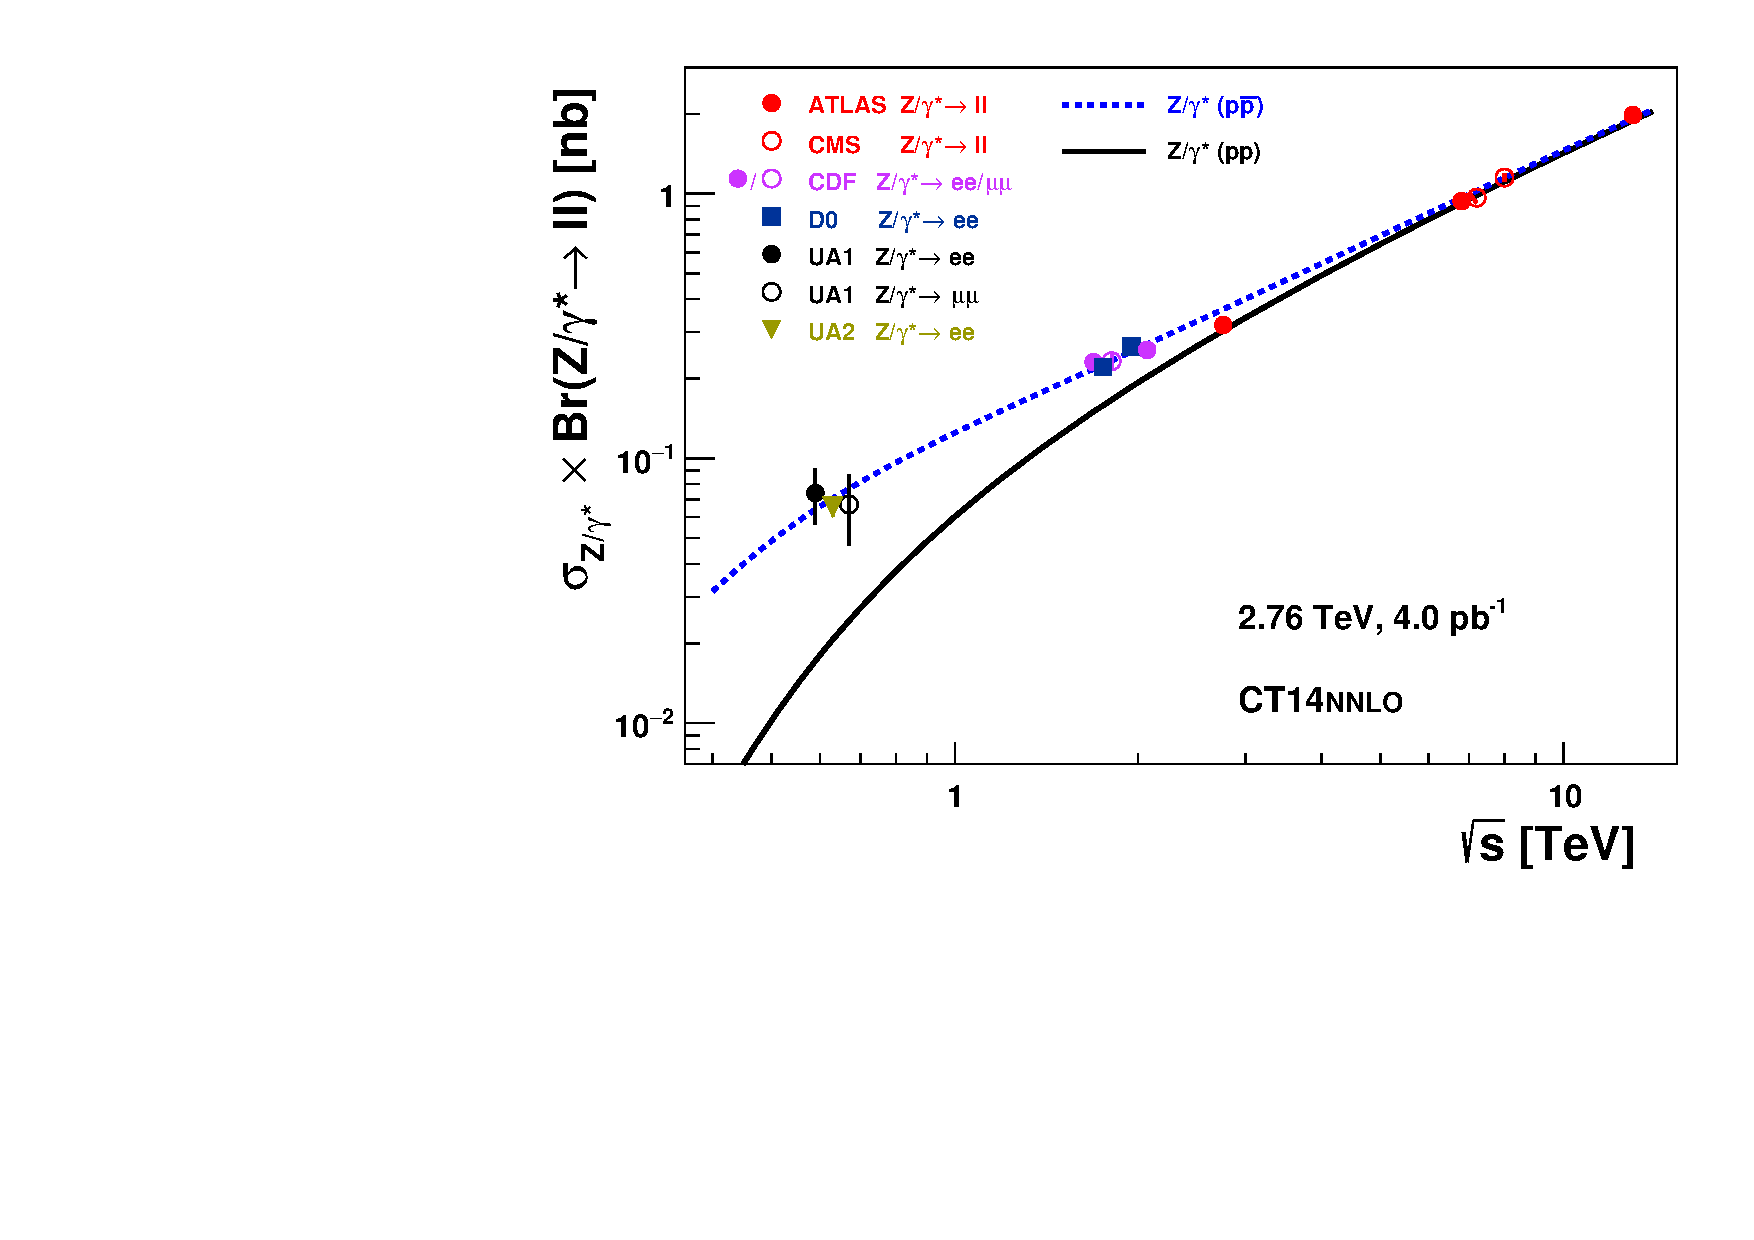
\includegraphics[width=0.7\linewidth]{Results/SigmaZatNNLOCombwithCMS.pdf} \\ b)}
\end{minipage}
\caption{The measured values of a) $\sigma_{W \to l\nu}$ for $W^+$, $W^-$ and  their sum and b) $\sigma_{Z \to ll}$ for Z-boson compared to the theoretical predictions based on NNLO QCD calculations. The ATLAS official results with addition of the 2.76 TeV measurement are shown for the combined electron-muon channel only . The predictions and previous measurements are shown for both proton-proton and proton-antiproton colliders as a function of $\sqrt{s}$. The data points at the various energies are staggered to improve readability. All data points are displayed with their total uncertainty. The calculations were performed with the program FEWZ using the CT14nnlo parton density function parameterization. The theoretical uncertainties on the cross section predictions are not shown.}
\label{fig:ZcsResults}
\end{figure}


\subsection{Cross section ratios}

Measurement of ratios is a powerful tool to test PDF predictions, since it allows for the cancellation of the biggest uncertainty coming from luminosity and reduce other sources of systematic uncertainties. The ratios of W and Z cross sections have been measured for 7 TeV\cite{a7TeV} and 13 TeV\cite{a13TeV} analyses. The measurement of the ratio $R_{W^{+}/W^{-}}$ is sensitive to the $u_{v}$, $d_{v}$ valence quarks distributions, while the ratio $R_{W/Z}$ can put a constrains on the strange quark distributions. The ratios for W/Z cross sections have been calculated in a fiducial region following the prescription from Sec.~\ref{sec:Rat}. For the electron channel analyses the ratios are:
\begin{center}
$R^{e}_{W/Z} = \valAelecWZ \pm \statAelecWZ \, (stat.)\, \pm \sysAelecWZ\, (sys.)$; \\
$R^{e}_{W^{+}/Z} = \valAelecWpZ \pm \statAelecWpZ\, (stat.)\, \pm \sysAelecWpZ \, (sys.)$; \\
$R^{e}_{W^{-}/Z} = \valAelecWmZ \pm \statAelecWmZ\, (stat.)\,  \pm \sysAelecWmZ\,  (sys.)$; \\
$R^{e}_{W^{+}/W^{-}} = \valAelecWpWm \pm \statAelecWpWm\, (stat.)\, \pm \sysAelecWpWm\,  (sys.)$\\
\end{center}
and for muon channel analyses:
\begin{center}
$R^{\mu}_{W/Z} = \valAmuonWZ \pm \statAmuonWZ \, (stat.)\, \pm \sysAmuonWZ\, (sys.)$;\\
$R^{\mu}_{W^{+}/Z} = \valAmuonWpZ \pm \statAmuonWpZ\, (stat.)\, \pm \sysAmuonWpZ \, (sys.)$; \\
$R^{\mu}_{W^{-}/Z} = \valAmuonWmZ \pm \statAmuonWmZ\, (stat.)\,  \pm \sysAmuonWmZ\,  (sys.)$;\\
$R^{\mu}_{W^{+}/W^{-}} = \valAmuonWpWm \pm \statAmuonWpWm\, (stat.)\, \pm \sysAmuonWpWm\,  (sys.)$.\\
\end{center}
The obtained results are in a good agreement with the combined channel results. The ratios calculated for the combined channel have reduced uncertainties:
\begin{center}
$R_{W/Z} = \valfidWZ \pm \statfidWZ \, (stat.)\, \pm \sysfidWZ\, (sys.)$; \\
$R_{W^{+}/Z} = \valfidWpZ \pm \statfidWpZ\, (stat.)\, \pm \sysfidWpZ \, (sys.)$; \\
$R_{W^{-}/Z} = \valfidWmZ \pm \statfidWmZ\, (stat.)\,  \pm \sysfidWmZ\,  (sys.)$; \\
$R_{W^{+}/W^{-}} = \valfidWpWm \pm \statfidWpWm\, (stat.)\, \pm \sysfidWpWm\,  (sys.)$. \\
\end{center}

\begin{figure}[!tbp]
\begin{minipage}[h]{0.45\linewidth}
\center{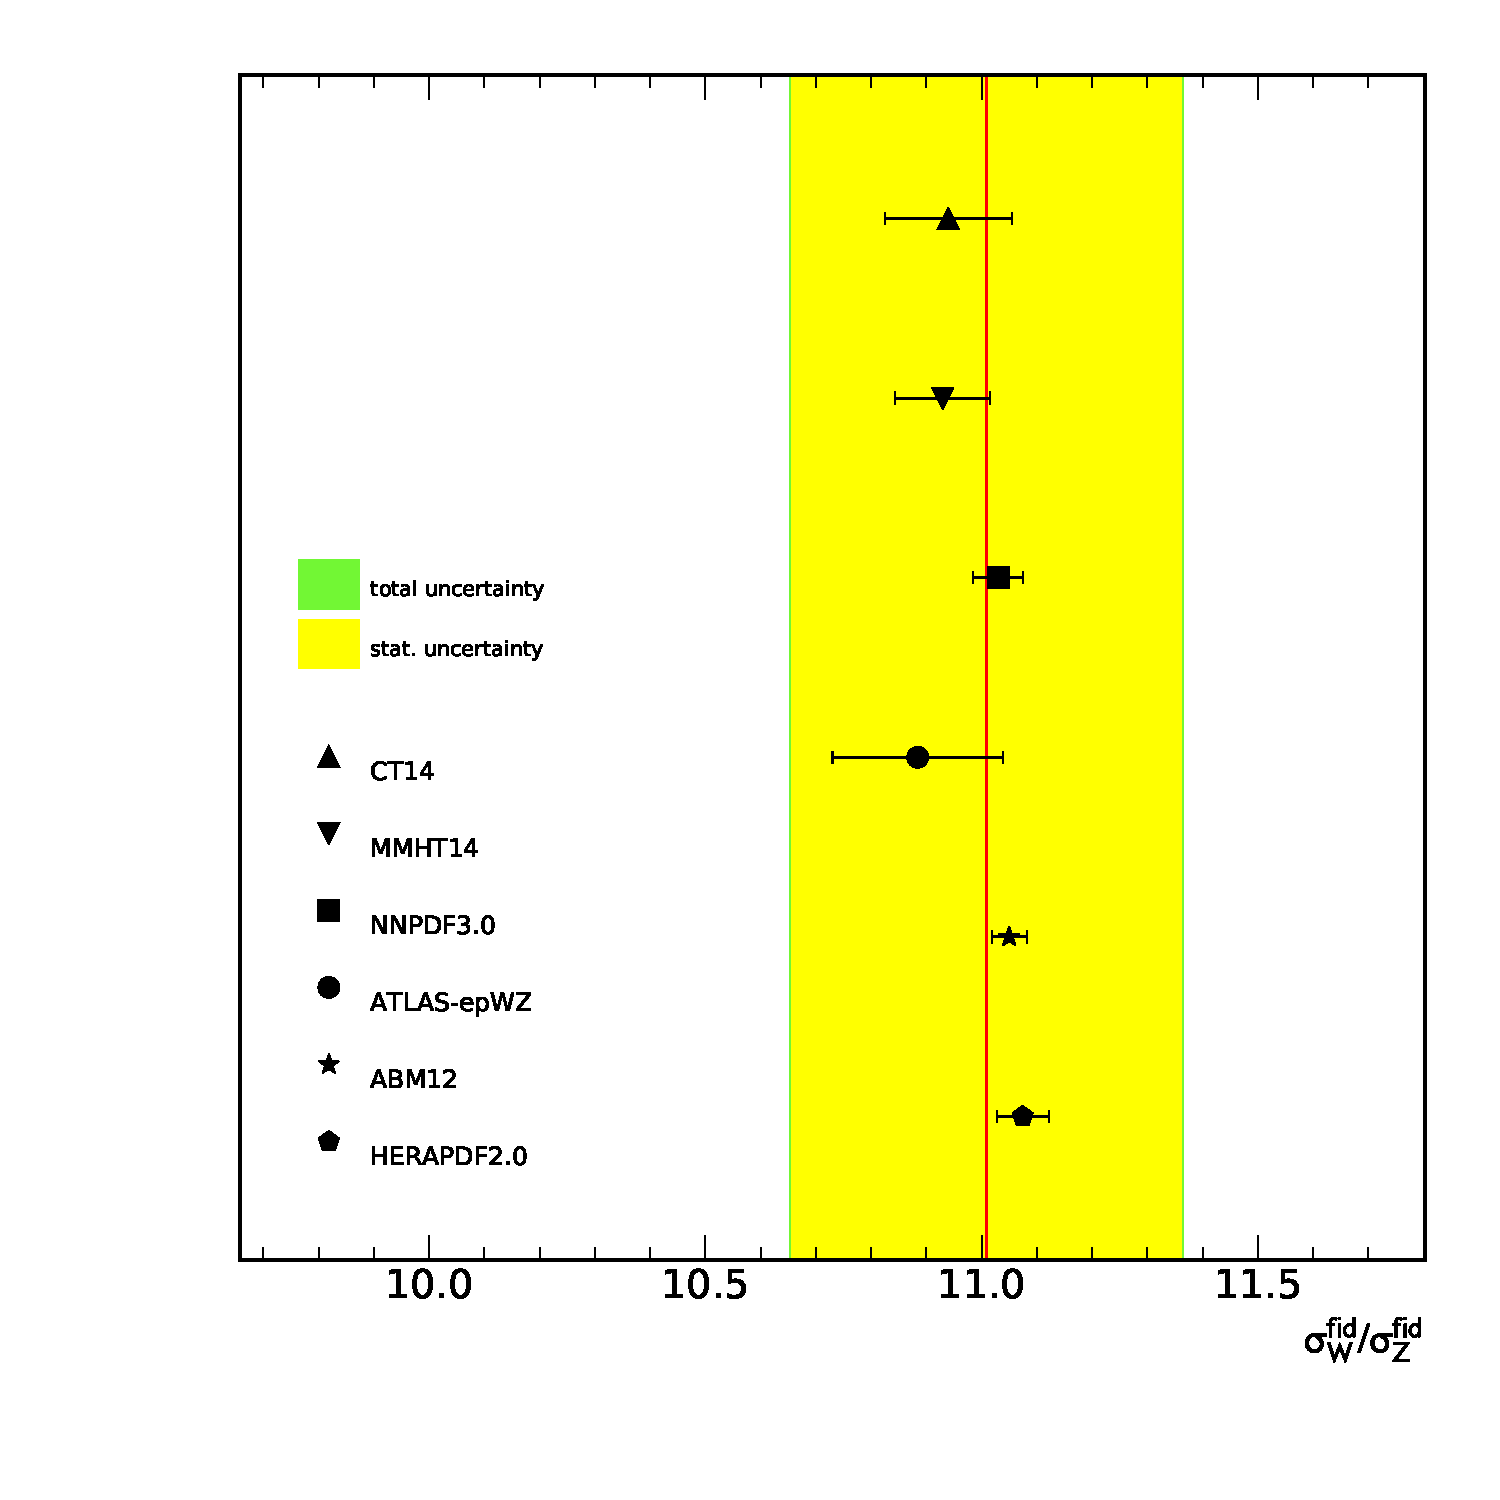
\includegraphics[width=1\textwidth]{Results/RatioWZ.pdf} \\ a)}
\end{minipage}
\hfill
\begin{minipage}[h]{0.45\linewidth}
\center{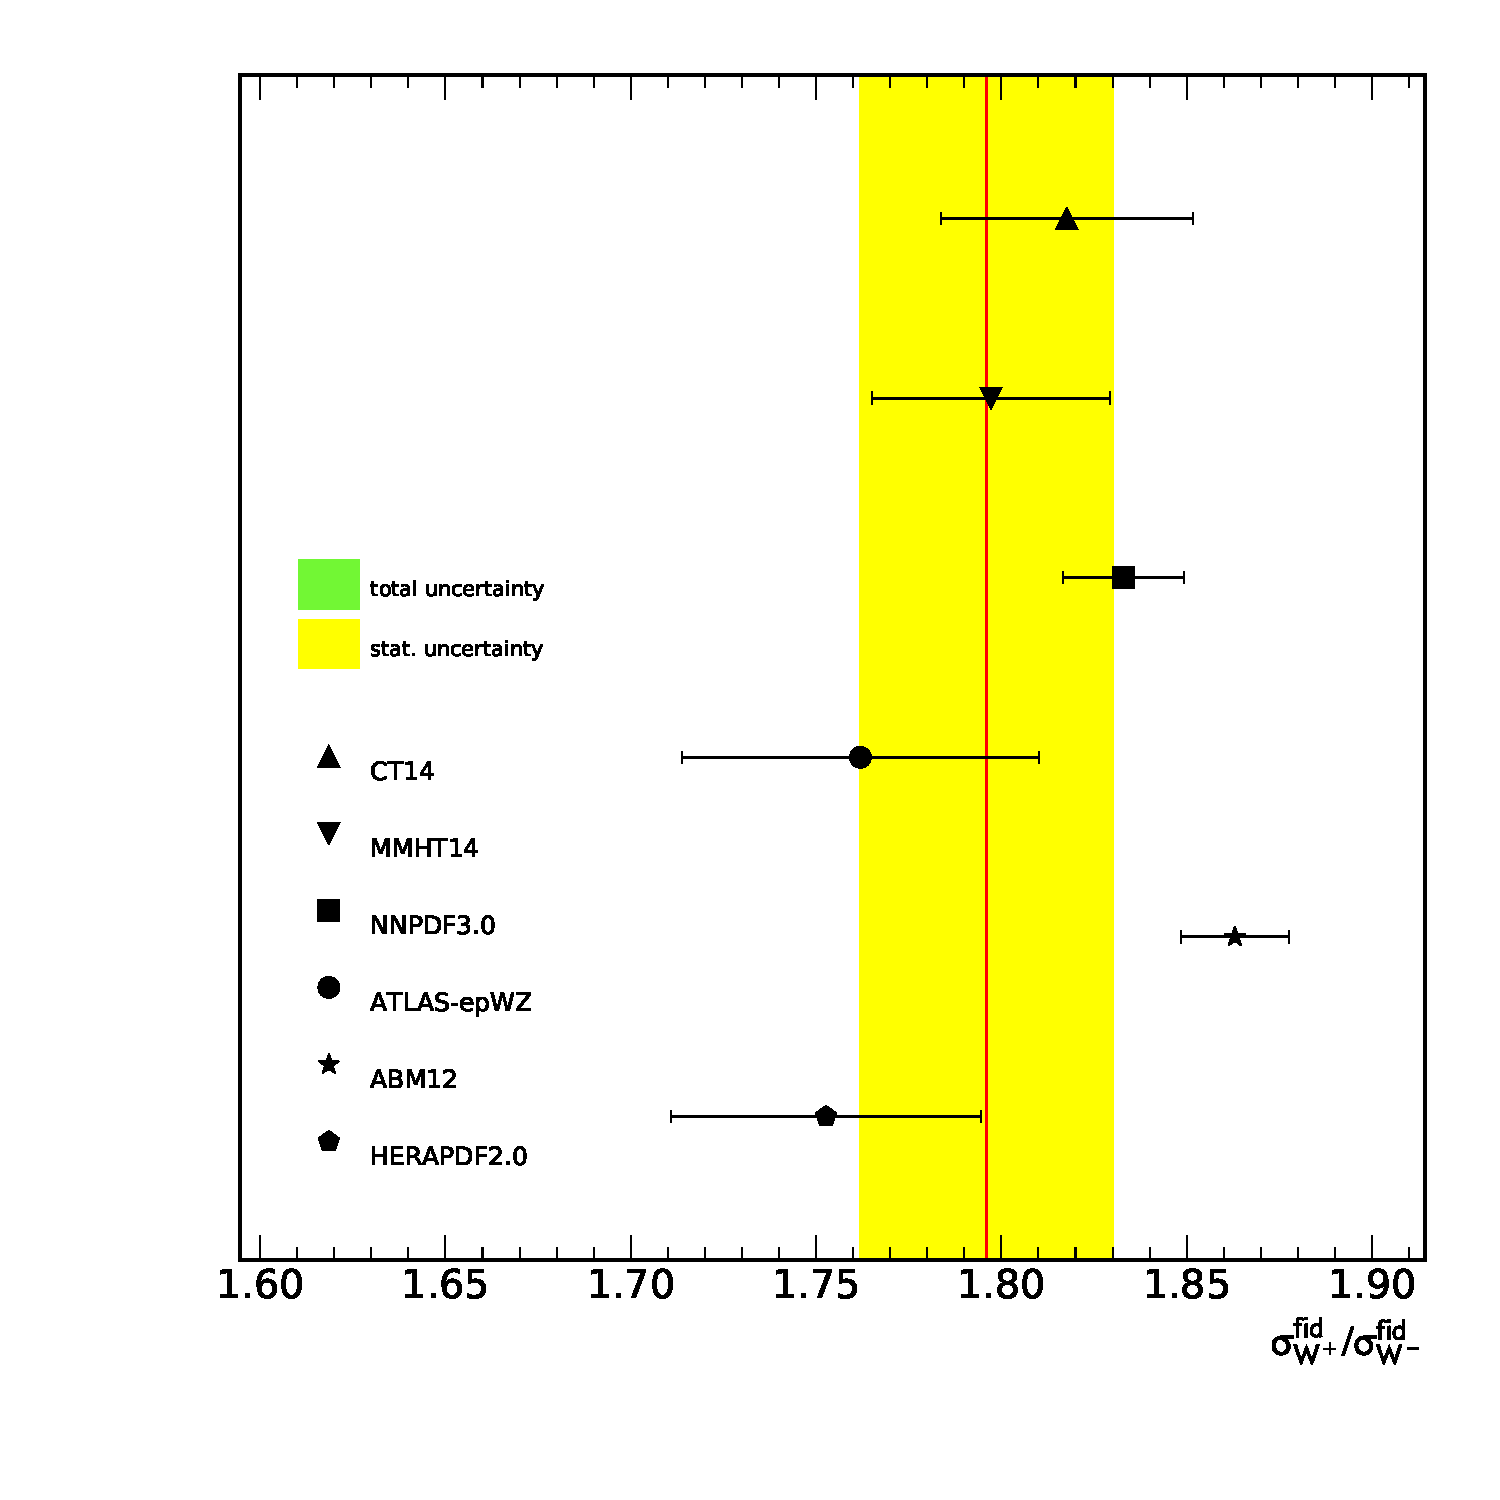
\includegraphics[width=1\textwidth]{Results/RatioWpWm.pdf}\\ b)}
\end{minipage}
\caption{Ratio of  a) W to Z  and b) $W^+$ to $W^-$ production fiducial cross sections compared to predictions based on the six pdf sets:  CT14nnlo, MMHT2014, NNPDF3.0, ATLASepWZ12, abm12, HERApdf2.0. The yellow band corresponds to the statistical uncertainty, while the systematic uncertainty is considered to be negligible. Theory predictions are given with the corresponding PDF uncertainties shown as error bands.}
\label{fig:WRatio}
\end{figure}

\begin{figure}[!tbp]
\begin{minipage}[h]{0.45\linewidth}
\center{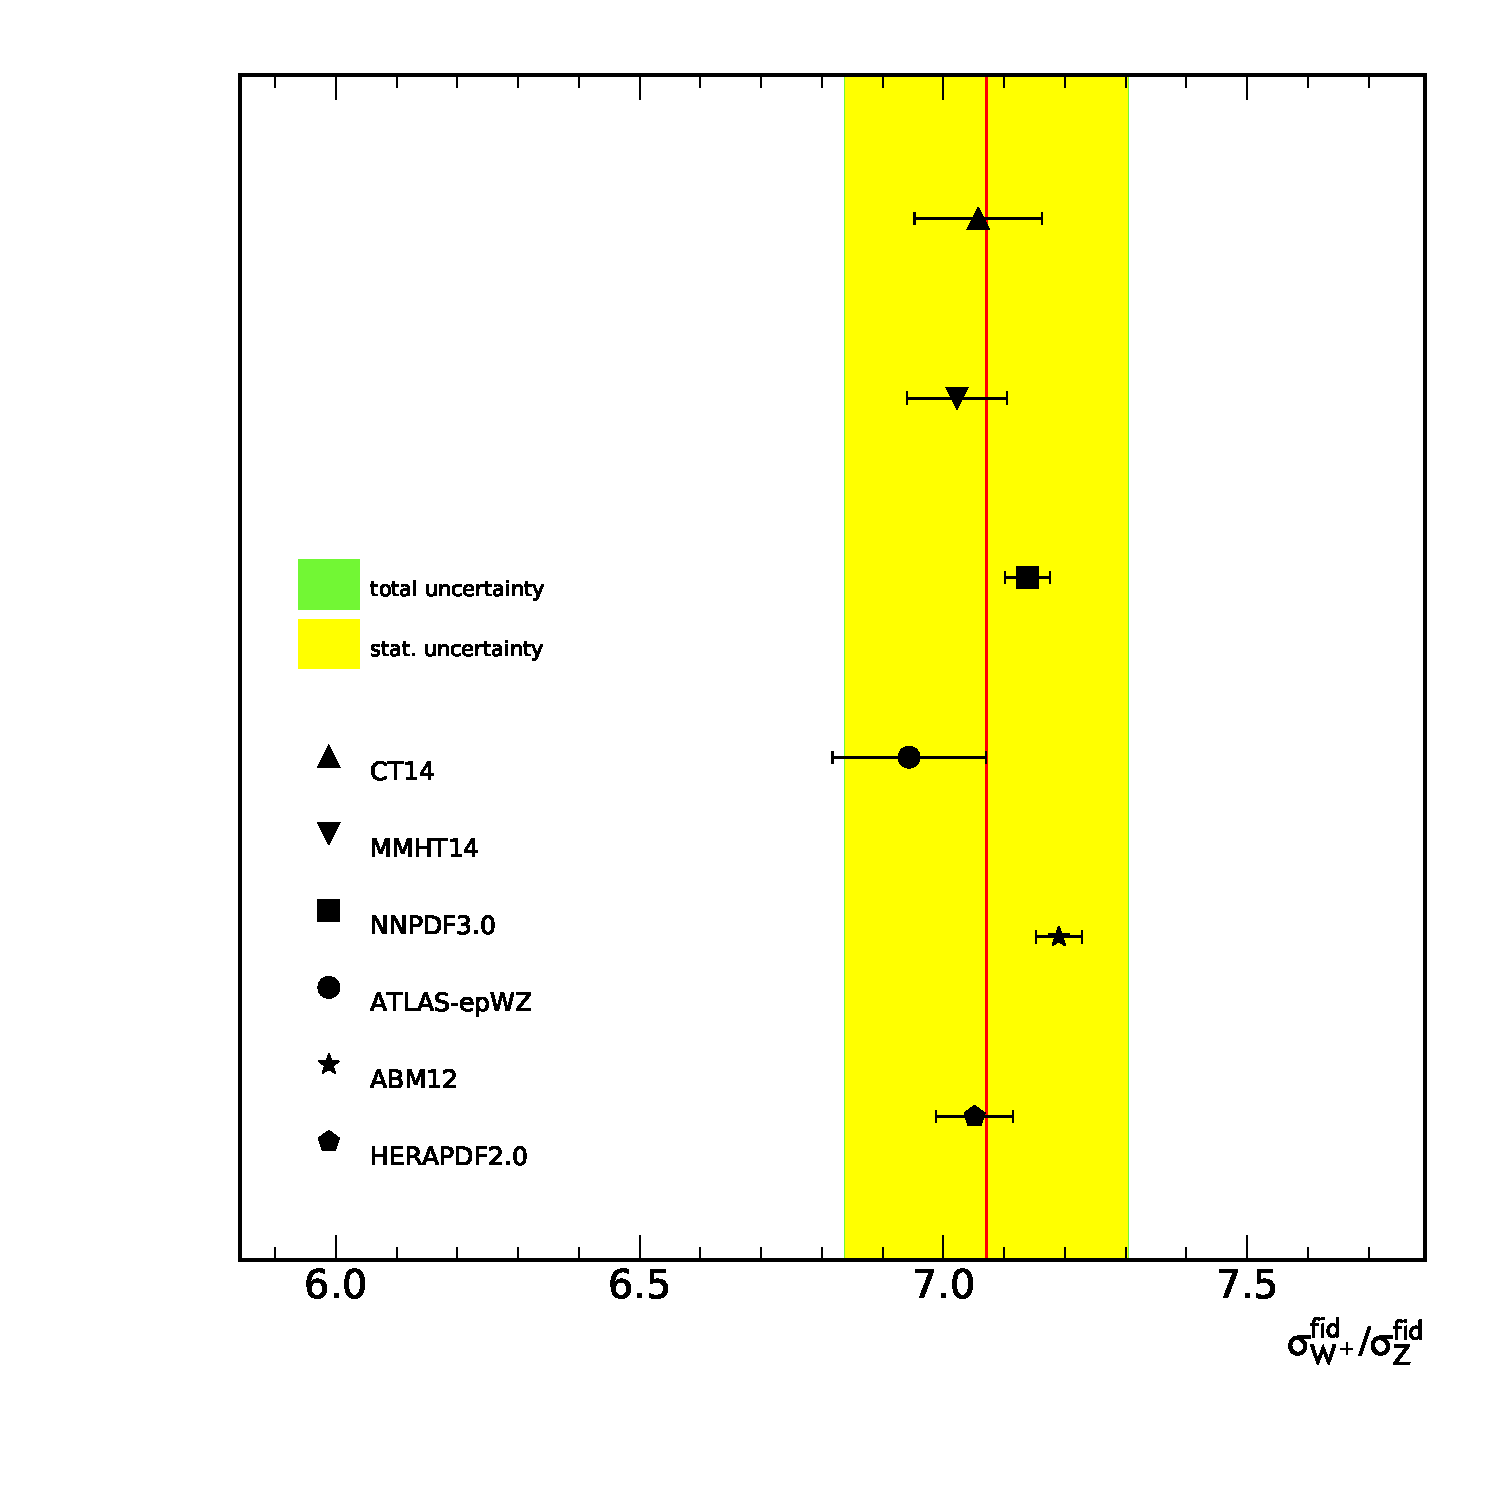
\includegraphics[width=1\textwidth]{Results/RatioWpZ.pdf} \\ a)}
\end{minipage}
\hfill
\begin{minipage}[h]{0.45\linewidth}
\center{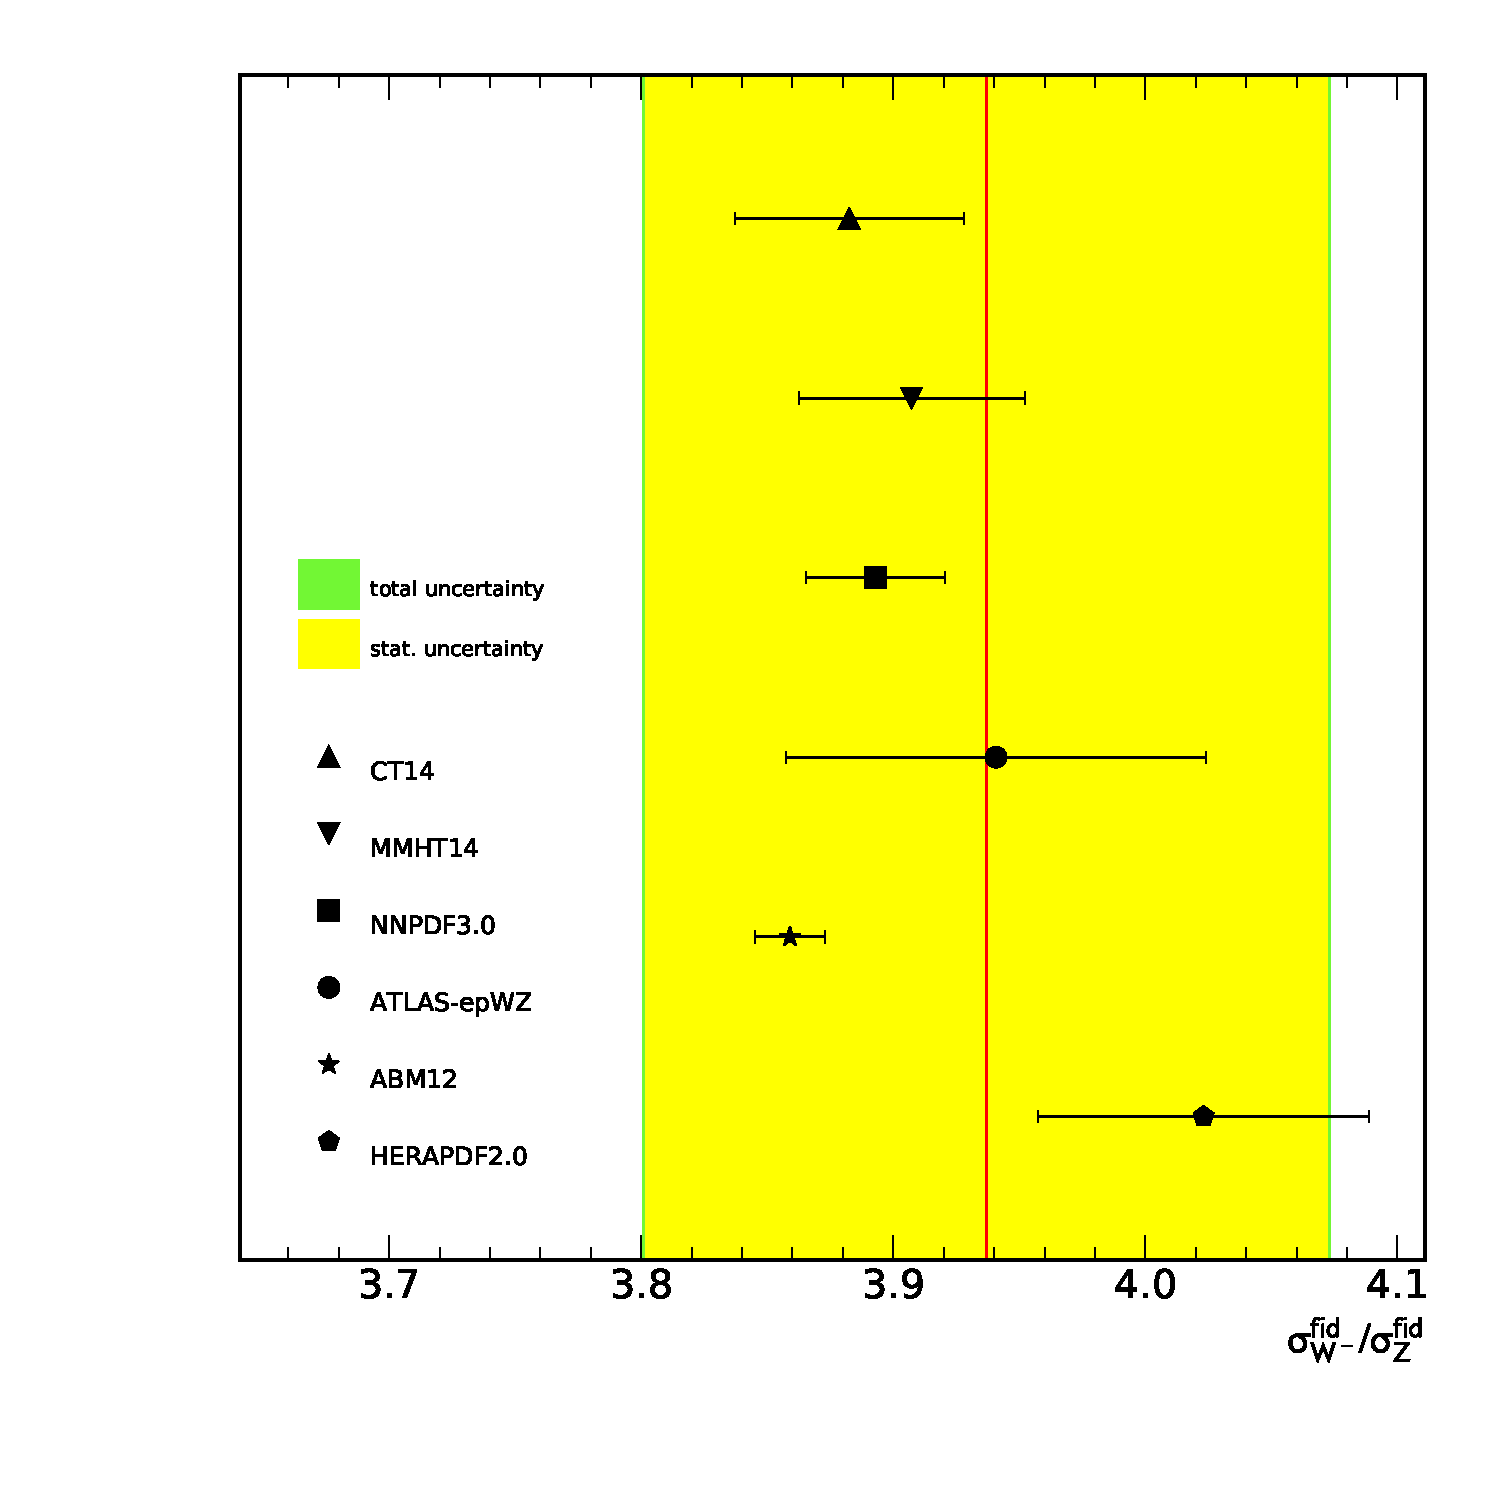
\includegraphics[width=1\textwidth]{Results/RatioWmZ.pdf} \\ b)}
\end{minipage}
\caption{Ratio of  a) $W^+$  to Z  and b) $W^-$ to Z production fiducial cross sections compared to predictions based on the six pdf sets:  CT14nnlo, MMHT2014, NNPDF3.0, ATLASepWZ12, abm12, HERApdf2.0. The yellow band corresponds to the statistical uncertainty, while the systematic uncertainty is considered to be negligible. Theory predictions are given with the corresponding PDF uncertainties shown as error bands.}
\label{fig:ZRatio}
\end{figure}

The resulting ratios are dominated by the statistical uncertainty. The ratios are agreeing withing the uncertainty between electron, muon and combined channel. The ratios for combined cross section are used to compare with NLO predictions (Fig.~\ref{fig:WRatio} and Fig.~\ref{fig:ZRatio}) for the six PDFs CT14nnlo, MMHT2014, NNPDF3.0, ATLASepWZ12, abm12, HERApdf2.0. Thanks to the higher statistics in the combined W-bosons analyses the ratio $R_{W^{+}/W^{-}}$ has the compatible to the PDF uncertainties. The ratios to the Z cross section $R_{W/Z}$, $R_{W^{+}/Z}$ and $R_{W^{-}/Z}$ are significantly less accurate because of the large statistical uncertainty of the Z cross section. The best agreement with the data is achieved by the MMHT PDF set.



\section{Effect on parton density functions}\label{sec:PDFCs}

The effect of inclusion of obtained cross sections in PDF set have been estimated using the profiling method, described in Sec.~\ref{sec:PDFFit}. As a reference, it was decided to use CT14 PDF set, because of its relatively good agreement with the data for both NLO and NNLO predictions. The profiling was performed at NLO order, however it is also possible to make NNLO profiling with use of the NNLO K-factors.

As it was mentioned in Chap.~\ref{chap:Theory} the measurement at 2.76 TeV is mostly sensitive to the valence $u_v$ and $d_v$, light-sea $\bar{d}$ and $\bar{u}$ quark distributions. The inclusion of 2.76 TeV cross sections in PDF can introduce both the reduction of the uncertainties of the PDF distributions and shift in the distributions. 

A sensitivity of this measurement to the PDF uncertainties have been studied by adding into the PDF set the $W$ and $Z$ cross sections scaled to match the theoretical predictions. This method does not introduce any shift in distributions, however makes a reduction of uncertainties more visible. The resulting distributions are shown in Fig.~\ref{fig:PDFSensitStrange} at the initial scale $Q^2=1.9$ GeV$^2$. This measurement allows to significantly reduce the uncertainties on $\bar{u}$ and $\bar{d}$ distributions. There is also a visible reduction of the uncertainties in the small x region for the valence quarks. Due to the limited statistics, the measurement cannot reduce the uncertainties on the strange quark distributions. As it was expected, the $W$ and $Z$ cross sections are not sensitive to the gluon density. It is possible to reduce the uncertainties on PDF distribution even more with inclusion of 5, 7 and 13 TeV $W$ and $Z$ cross sections, because of the large number of correlated uncertainties for a different energy measurements (especially luminosity).

The full profiling results are shown in Fig.~\ref{fig:PDFValenceShift}-~\ref{fig:PDFSeaShift}. The initial value of $\chiD/NDF$=1.2/3 shows a good agreement with theoretical predictions, however the fit allows to reduce it to the further to the value $\chiD/NDF$=0.8/3. The profiling procedure introduces a shift in $u_v$, $d_v$, $\bar{u}$, $\bar{v}$, $s$ quark distributions within 1 sigma.  The gluon distribution is left unchanged. The additional PDF profiling plots can be found in Appendix~\ref{app:PDF}.

The predictions of the obtained profiled CT14 set are shown in Fig.~\ref{fig:PDFEffectXsec}-~\ref{fig:PDFEffectRatio}. The cross sections, predicted by the profiled CT14 set are in a better, however not perfect, agreement with the data, compared to the original set. There is also a small reduction of the uncertainties.

\begin{figure}[!tbp]
\begin{minipage}[h]{0.4\linewidth}
\center{\includegraphics[width=1\textwidth]{Results/Sensitivity/uv_ratio.pdf} \\ a)}
\end{minipage}
\hfill
\begin{minipage}[h]{0.4\linewidth}
\center{\includegraphics[width=1\textwidth]{Results/Sensitivity/dv_ratio.pdf} \\ b)}
\end{minipage}
\vfill
\begin{minipage}[h]{0.4\linewidth}
\center{\includegraphics[width=1\textwidth]{Results/Sensitivity/UBar_ratio.pdf} \\ c)}
\end{minipage}
\hfill
\begin{minipage}[h]{0.4\linewidth}
\center{\includegraphics[width=1\textwidth]{Results/Sensitivity/DBar_ratio.pdf} \\ d)}
\end{minipage}
\vfill
\begin{minipage}[h]{0.4\linewidth}
\center{\includegraphics[width=1\textwidth]{Results/Sensitivity/s_ratio.pdf} \\ e)}
\end{minipage}
\hfill
\begin{minipage}[h]{0.4\linewidth}
\center{\includegraphics[width=1\textwidth]{Results/Sensitivity/g_ratio.pdf} \\ f)}
\end{minipage}
\caption{Relative experimental uncertainties for the quark and gluon densities as a function of $x$ at scale $Q^2=$ 1.9 GeV$^2$. The red band denotes the reference NLO PDF distributions from CT14 pdf set. The impact of the addition of the new W,Z cross sections at 2.76 TeV on the PDF set uncertainties is shown by the blue boundaries.}
\label{fig:PDFSensitStrange}
\end{figure}

\begin{figure}[!tbp]
\begin{minipage}[h]{0.4\linewidth}
\center{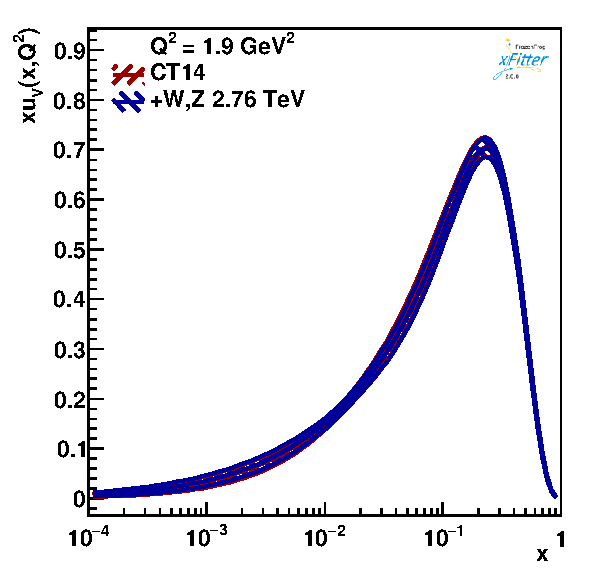
\includegraphics[width=1\textwidth]{Results/Shift/uv.pdf} \\ a)}
\end{minipage}
\hfill
\begin{minipage}[h]{0.4\linewidth}
\center{\includegraphics[width=1\textwidth]{Results/Shift/uv_ratio.pdf} \\ b)}
\end{minipage}
\vfill
\begin{minipage}[h]{0.4\linewidth}
\center{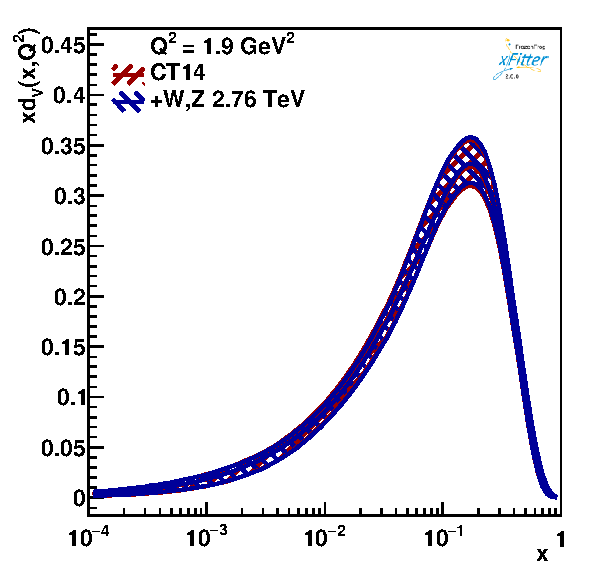
\includegraphics[width=1\textwidth]{Results/Shift/dv.pdf} \\ c)}
\end{minipage}
\hfill
\begin{minipage}[h]{0.4\linewidth}
\center{\includegraphics[width=1\textwidth]{Results/Shift/dv_ratio.pdf} \\ d)}
\end{minipage}
\vfill
\begin{minipage}[h]{0.4\linewidth}
\center{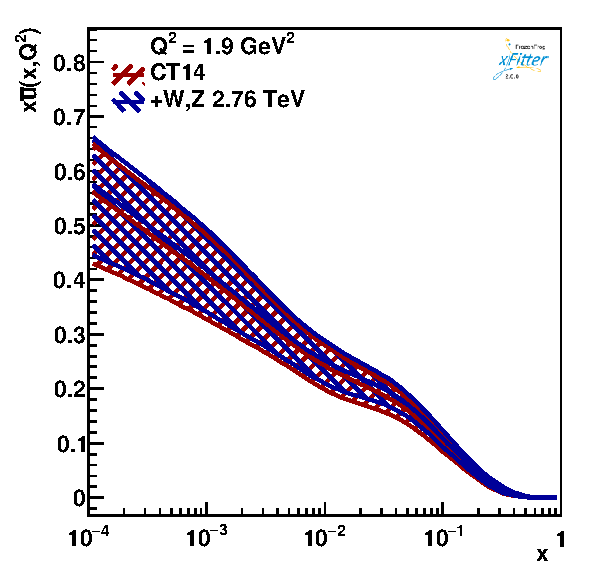
\includegraphics[width=1\textwidth]{Results/Shift/UBar.pdf} \\ e)}
\end{minipage}
\hfill
\begin{minipage}[h]{0.4\linewidth}
\center{\includegraphics[width=1\textwidth]{Results/Shift/UBar_ratio.pdf} \\ f)}
\end{minipage}
\caption{Absolute and  relative distributions for the $u_v$, $d_v$, $\bar{u}$ quark densities as a function of $x$ at scale $Q^2=$ 1.9 GeV$^2$ with the experimental uncertainties. The red band denotes the reference NLO PDF distributions from CT14 pdf set. The impact of the addition of the new W,Z cross sections at 2.76 TeV on the PDF set is shown by the blue boundaries.}
\label{fig:PDFValenceShift}
\end{figure}

\begin{figure}[!tbp]
\begin{minipage}[h]{0.4\linewidth}
\center{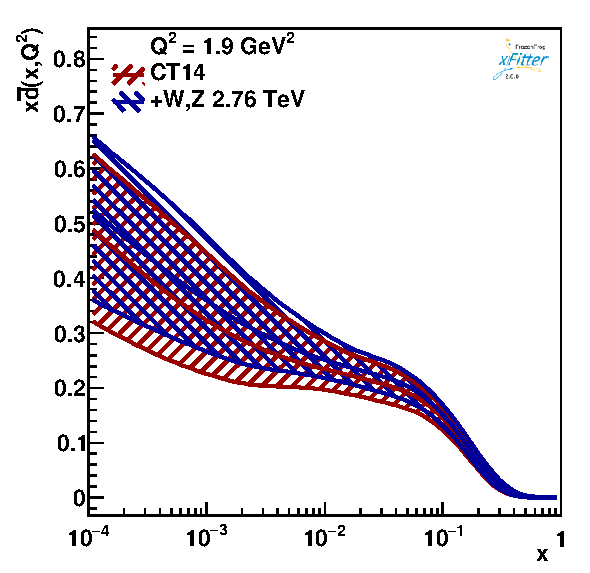
\includegraphics[width=1\textwidth]{Results/Shift/DBar.pdf} \\ a)}
\end{minipage}
\hfill
\begin{minipage}[h]{0.4\linewidth}
\center{\includegraphics[width=1\textwidth]{Results/Shift/DBar_ratio.pdf} \\ b)}
\end{minipage}
\vfill
\begin{minipage}[h]{0.4\linewidth}
\center{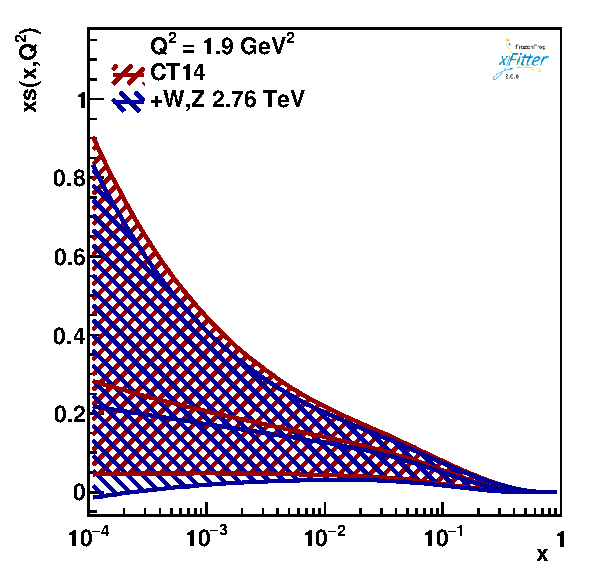
\includegraphics[width=1\textwidth]{Results/Shift/s.pdf} \\ c)}
\end{minipage}
\hfill
\begin{minipage}[h]{0.4\linewidth}
\center{\includegraphics[width=1\textwidth]{Results/Shift/s_ratio.pdf} \\ d)}
\end{minipage}
\vfill
\begin{minipage}[h]{0.4\linewidth}
\center{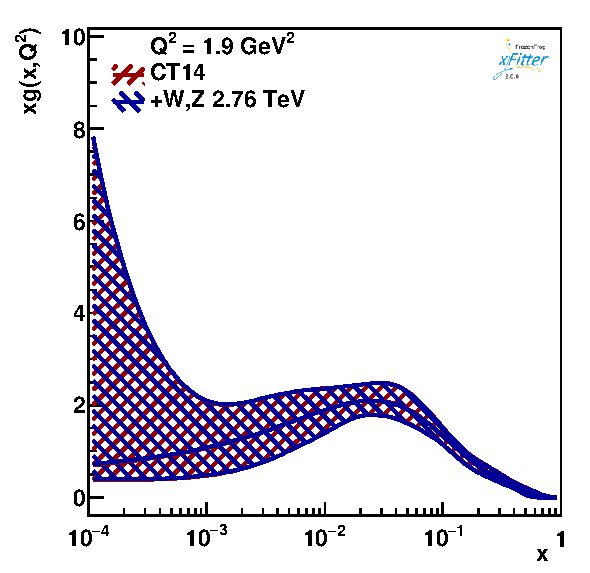
\includegraphics[width=1\textwidth]{Results/Shift/g.pdf} \\ e)}
\end{minipage}
\hfill
\begin{minipage}[h]{0.4\linewidth}
\center{\includegraphics[width=1\textwidth]{Results/Shift/g_ratio.pdf} \\ f)}
\end{minipage}
\caption{Absolute and  relative distributions for the $\bar{d}$ and $s$ quark and gluon densities as a function of $x$ at scale $Q^2=$ 1.9 GeV$^2$ with the experimental uncertainties. The red band denotes the reference NLO PDF distributions from CT14 pdf set. The impact of the addition of the new W,Z cross sections at 2.76 TeV on the PDF set is shown by the blue boundaries.}
\label{fig:PDFSeaShift}
\end{figure}


%\begin{figure}[!tbp]
%\begin{center}
%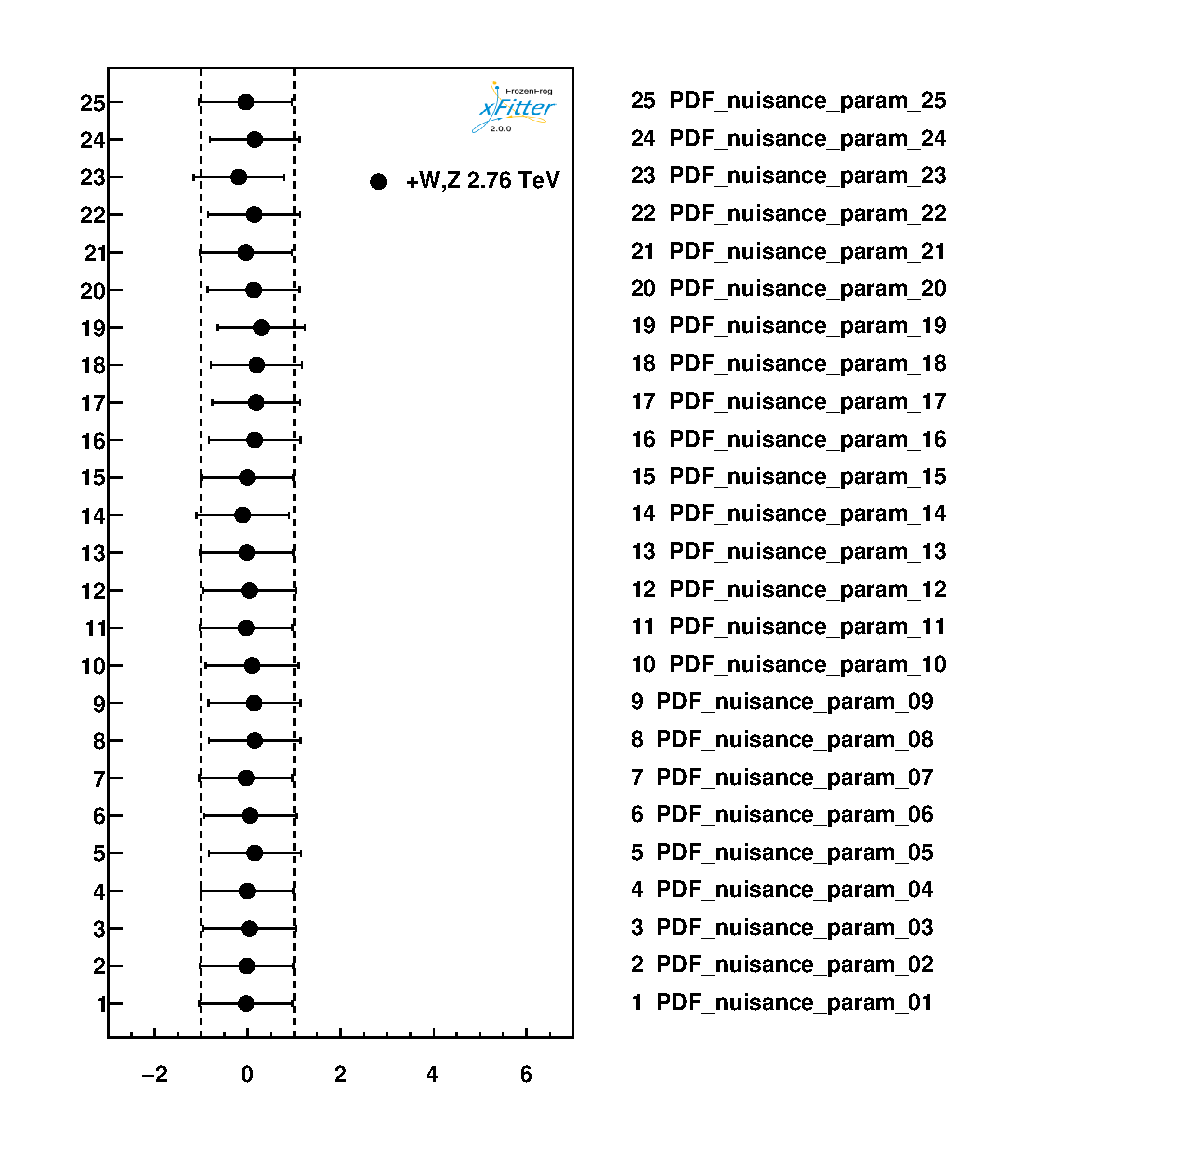
\includegraphics[width=0.7\textwidth]{Results/shifts_0.pdf}
%\end{center}
%\caption{Relative shift in PDF nuisance parameters due to the PDF profiling}
%\label{fig:shiftPDF}
%\end{figure}

\begin{figure}[!tbp]
\begin{minipage}[h]{0.32\linewidth}
\center{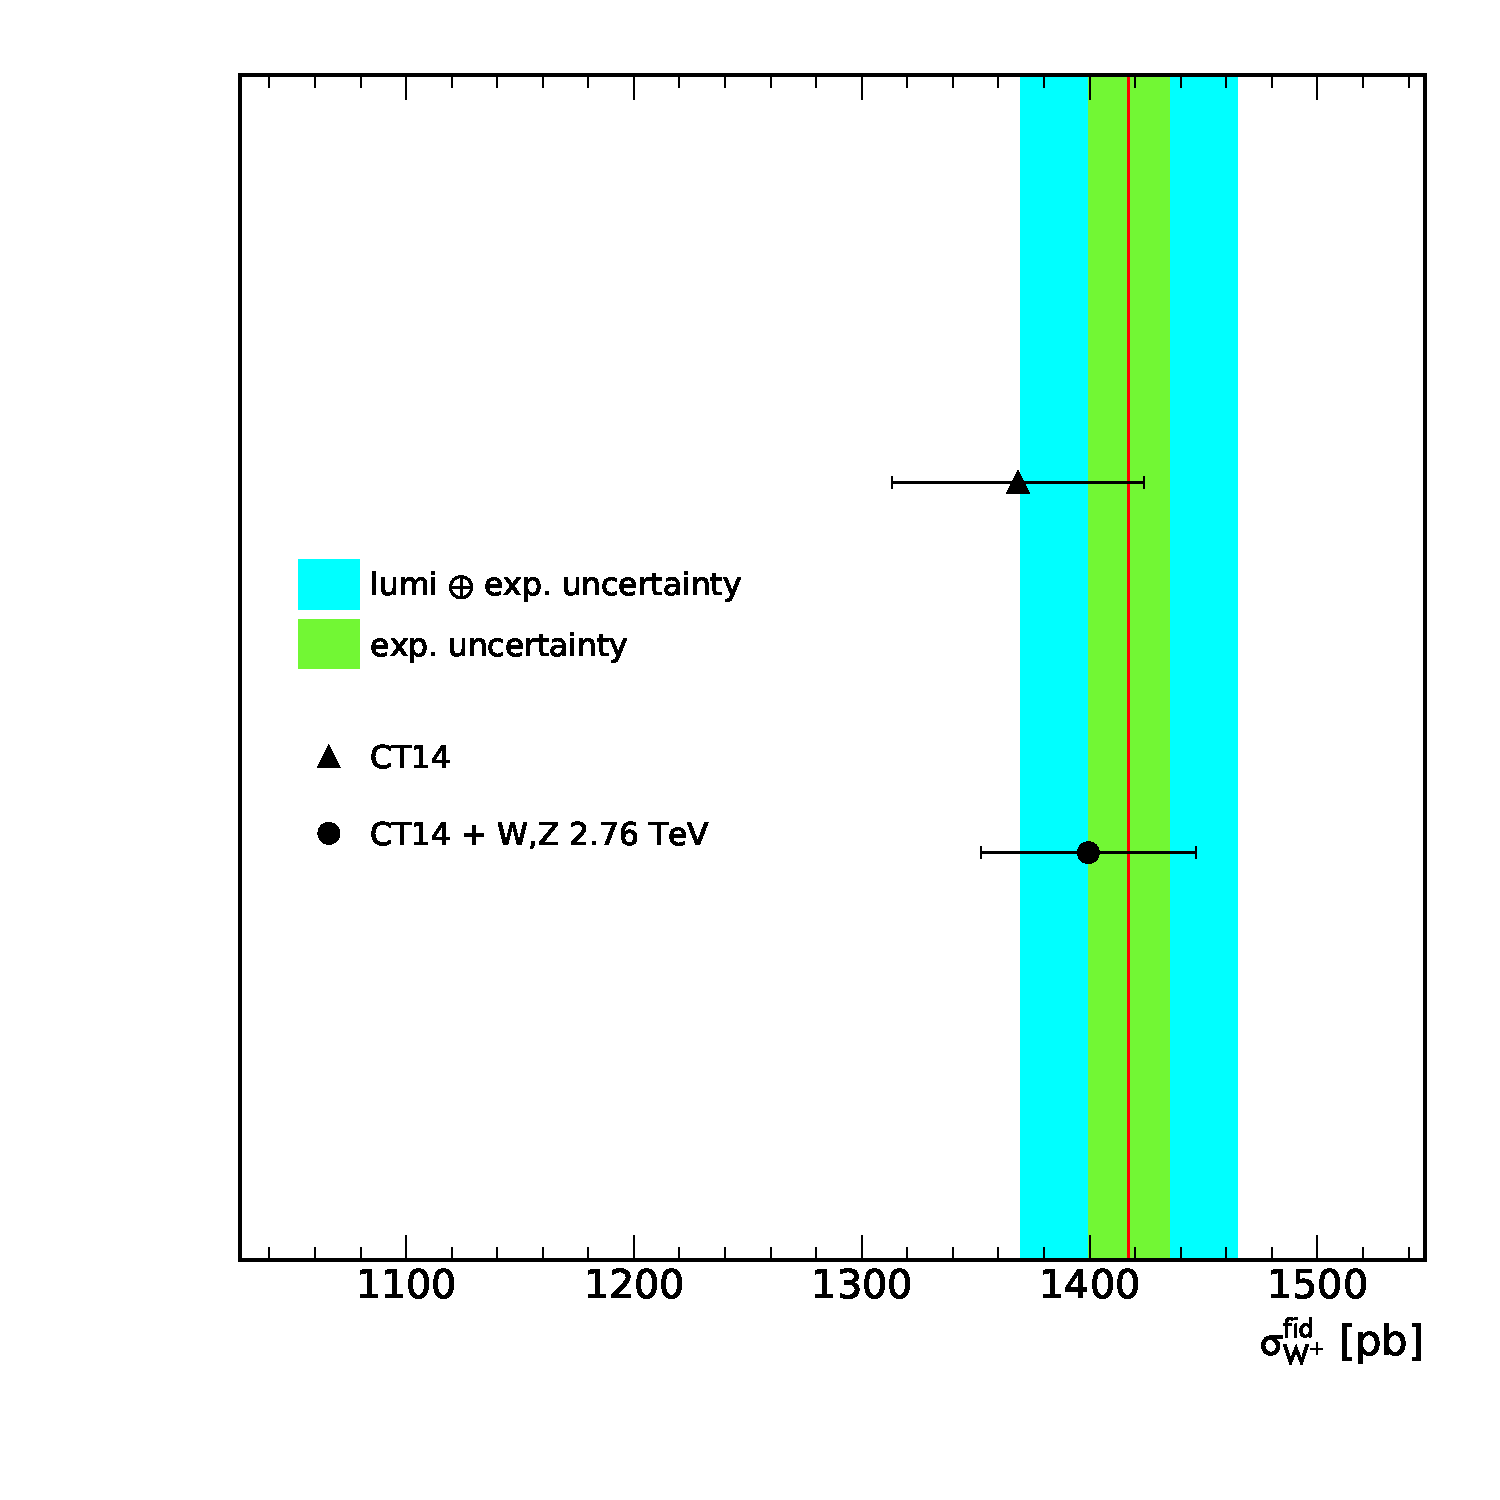
\includegraphics[width=1\textwidth]{Results/PDFImpWPlus.pdf} \\ a)}
\end{minipage}
\hfill
\begin{minipage}[h]{0.32\linewidth}
\center{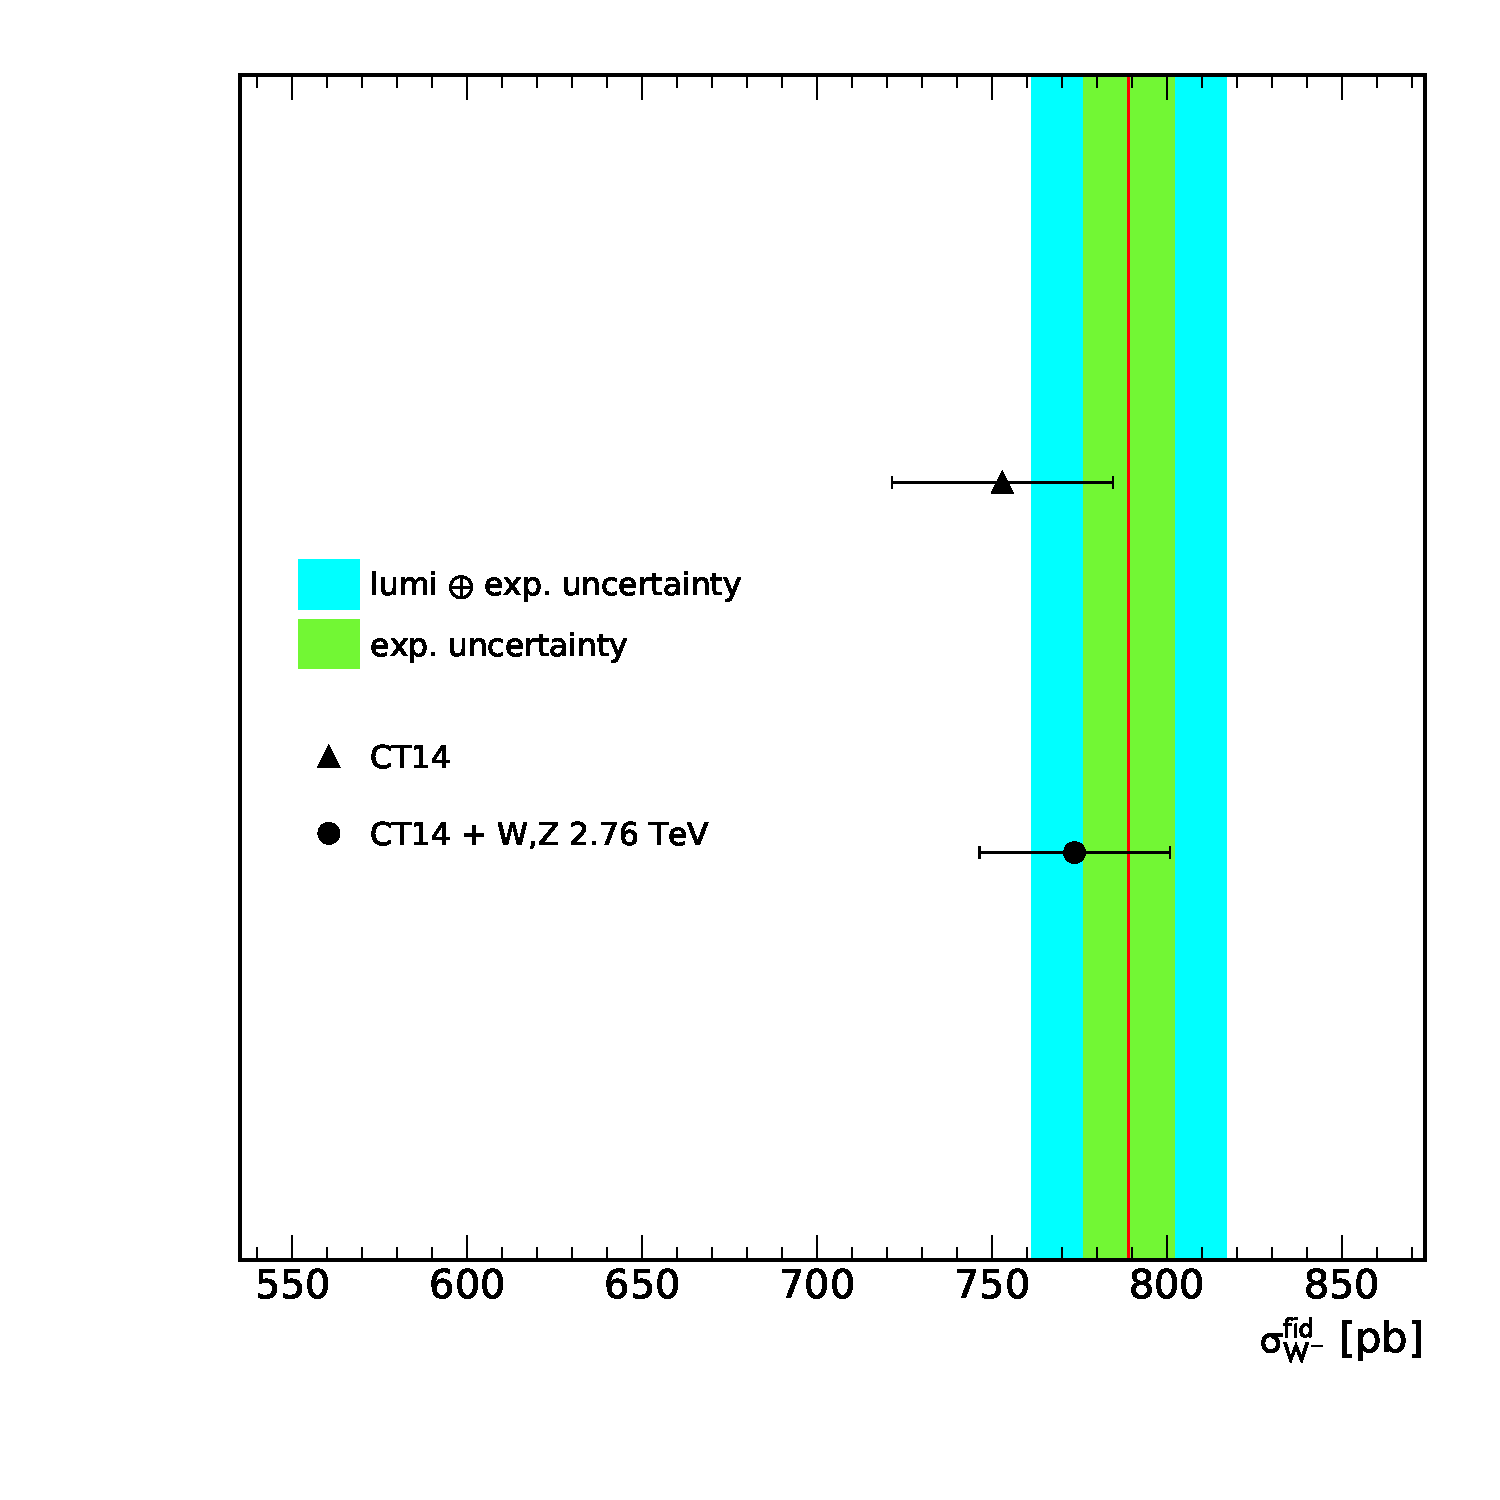
\includegraphics[width=1\textwidth]{Results/PDFImpWMinus.pdf} \\ b)}
\end{minipage}
\hfill
\begin{minipage}[h]{0.32\linewidth}
\center{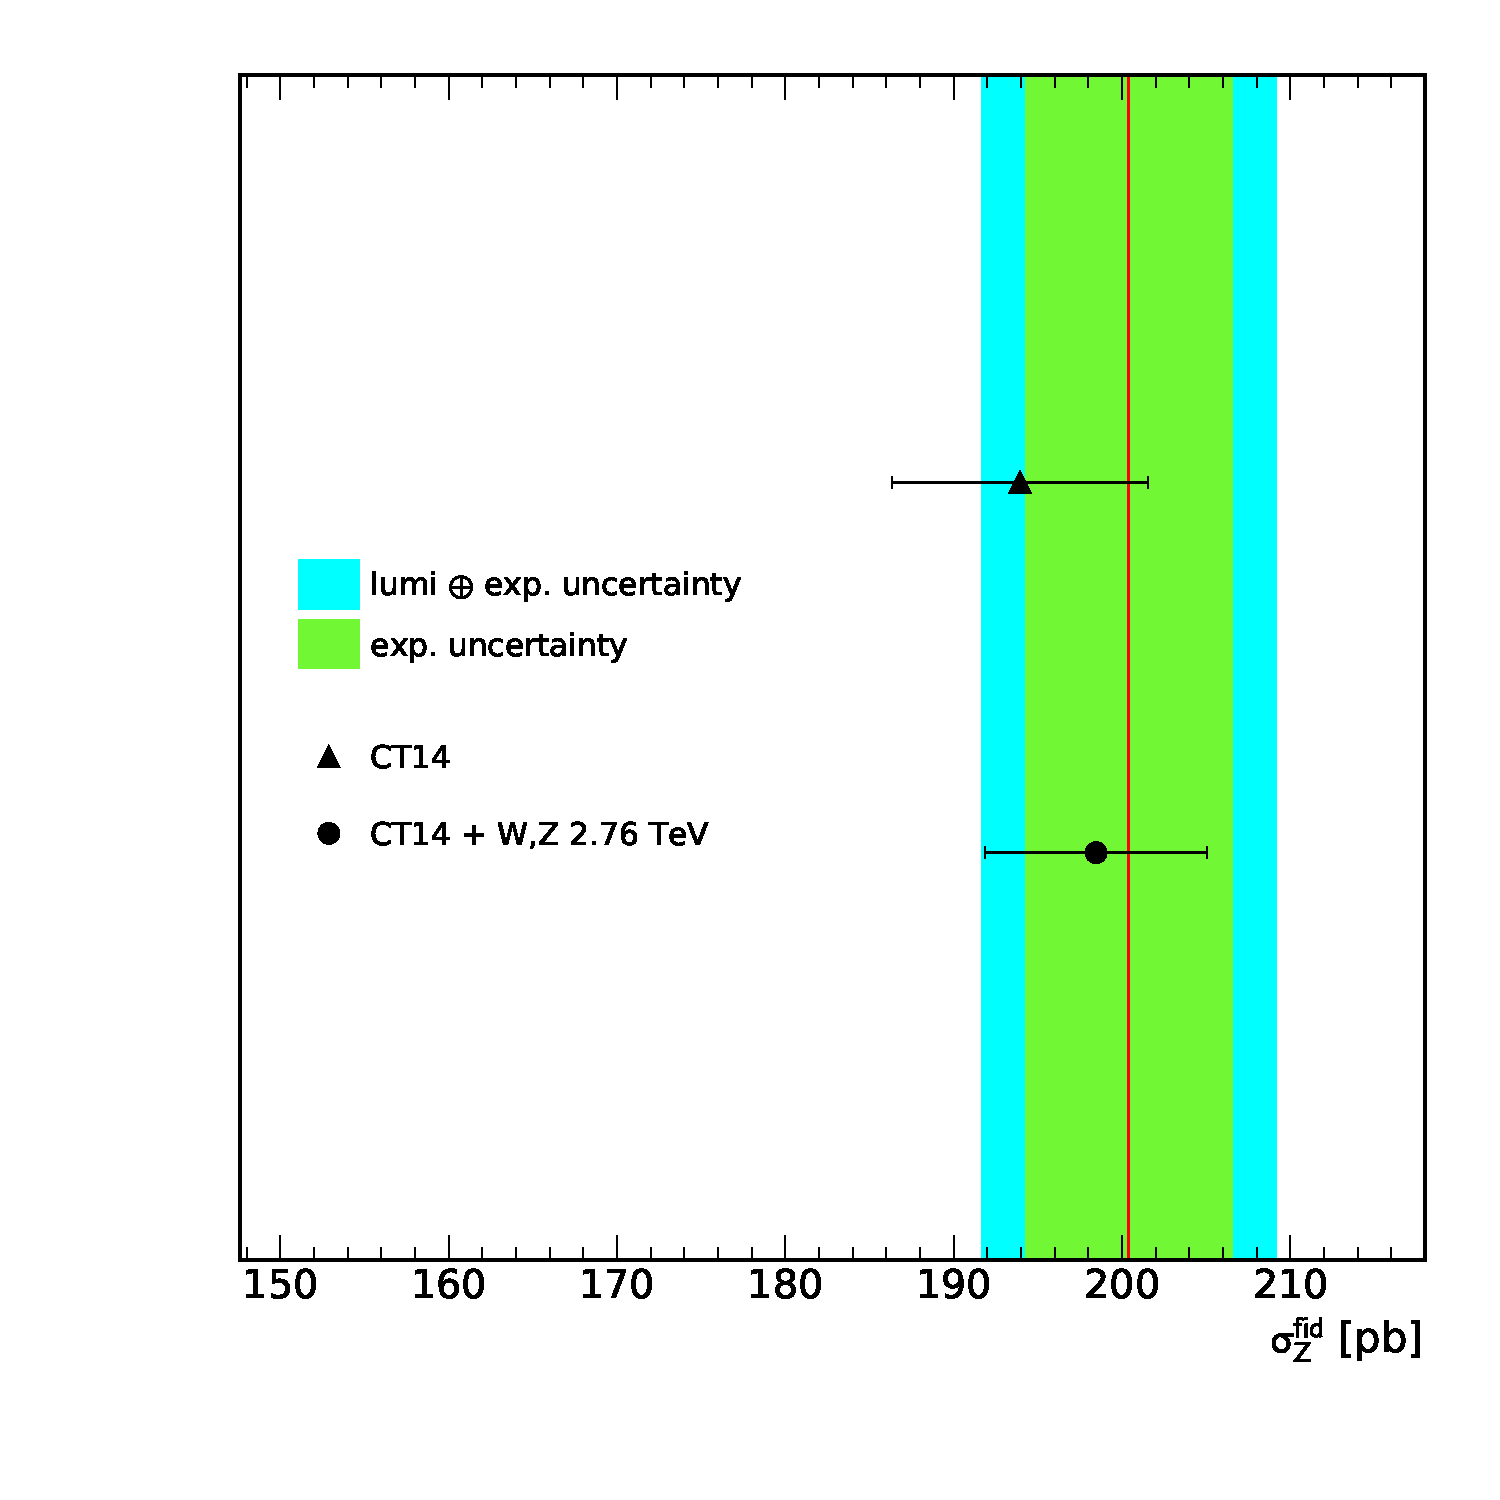
\includegraphics[width=1\textwidth]{Results/PDFImpZ.pdf} \\ c)}
\end{minipage}
\caption{The measured a) $W^{+}$,  b) $W^-$ and c) $Z$ production fiducial cross sections in combined channel compared to NLO predictions based on the original and profiled CT14 PDF set.}
\label{fig:PDFEffectXsec}
\end{figure}



\begin{figure}[!tbp]
\begin{minipage}[h]{0.49\linewidth}
\center{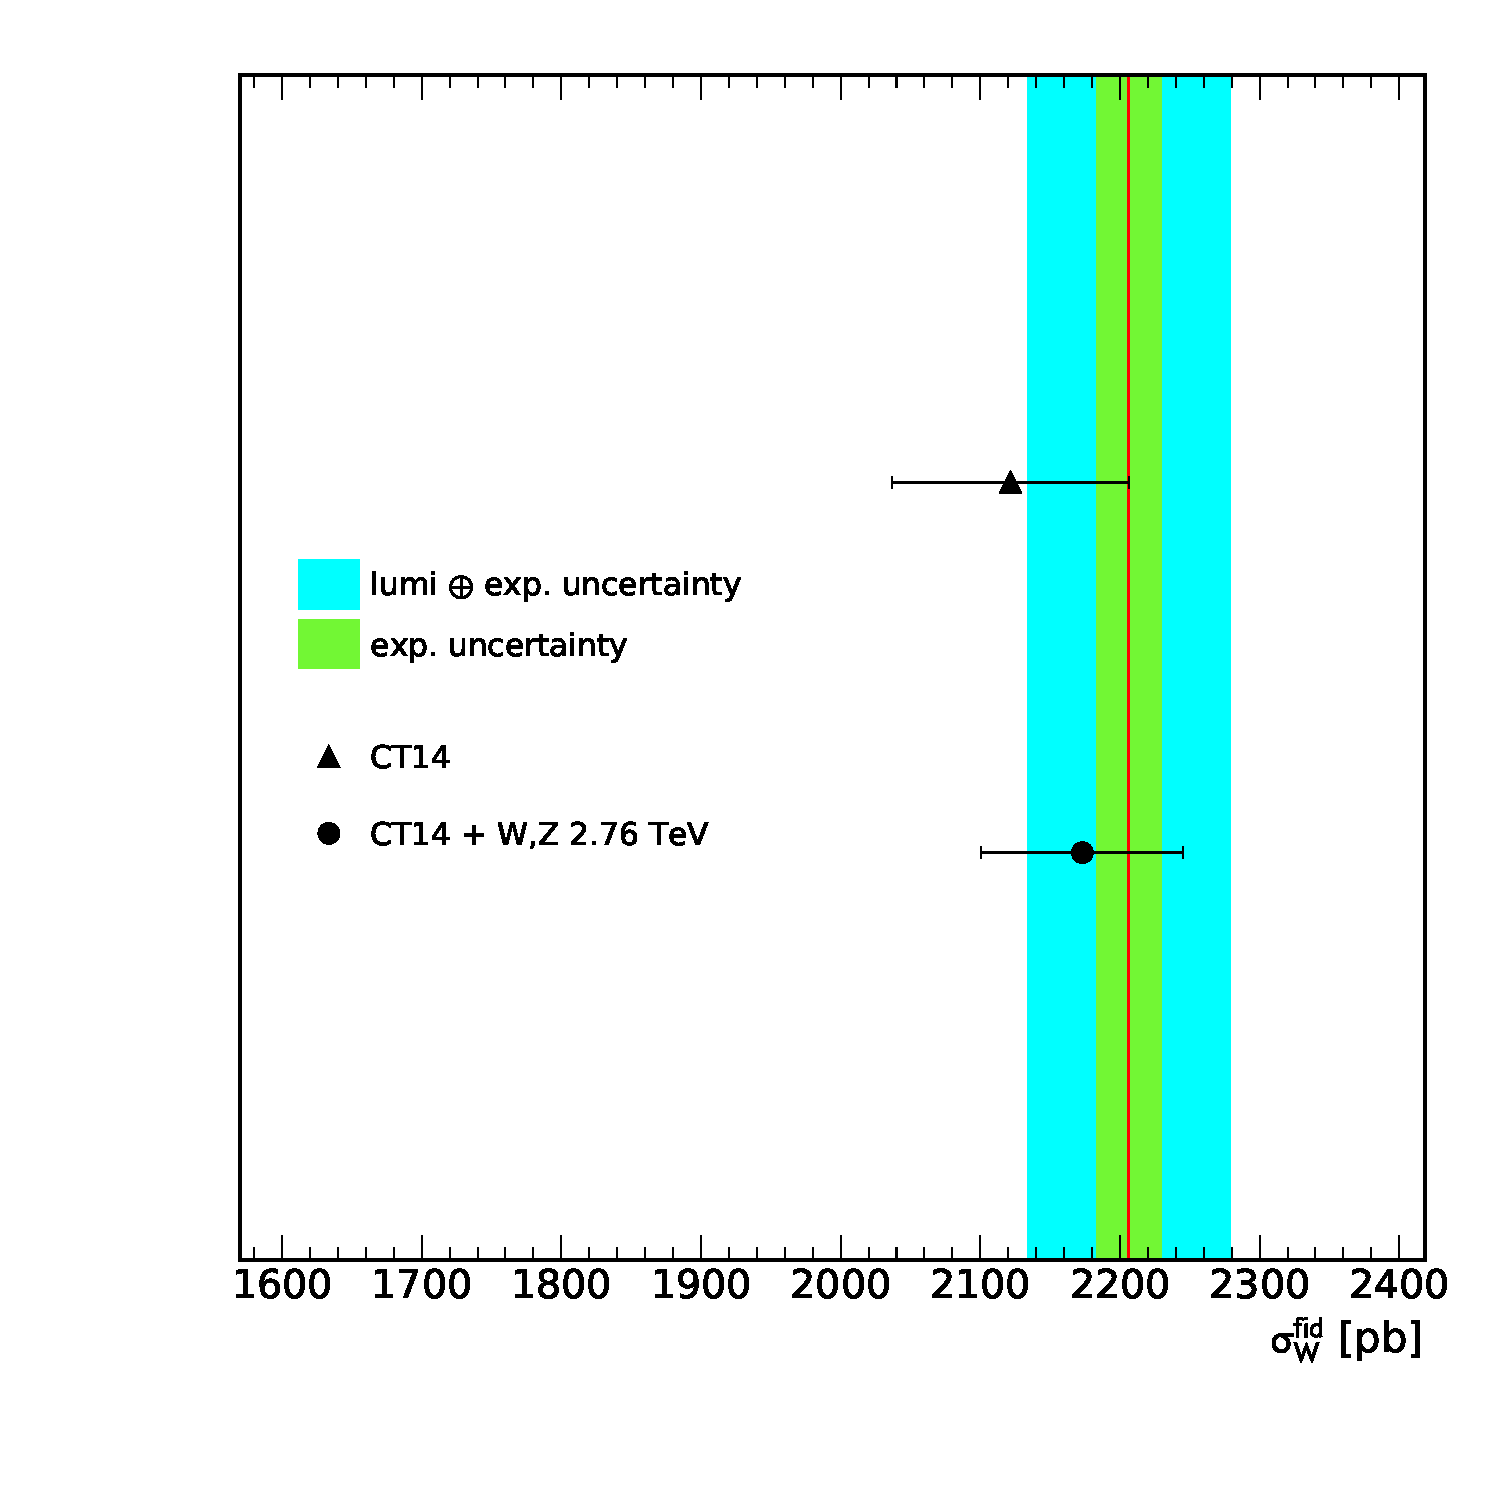
\includegraphics[width=1\textwidth]{Results/PDFImpW.pdf} \\ c)}
\end{minipage}
\begin{minipage}[h]{0.49\linewidth}
\center{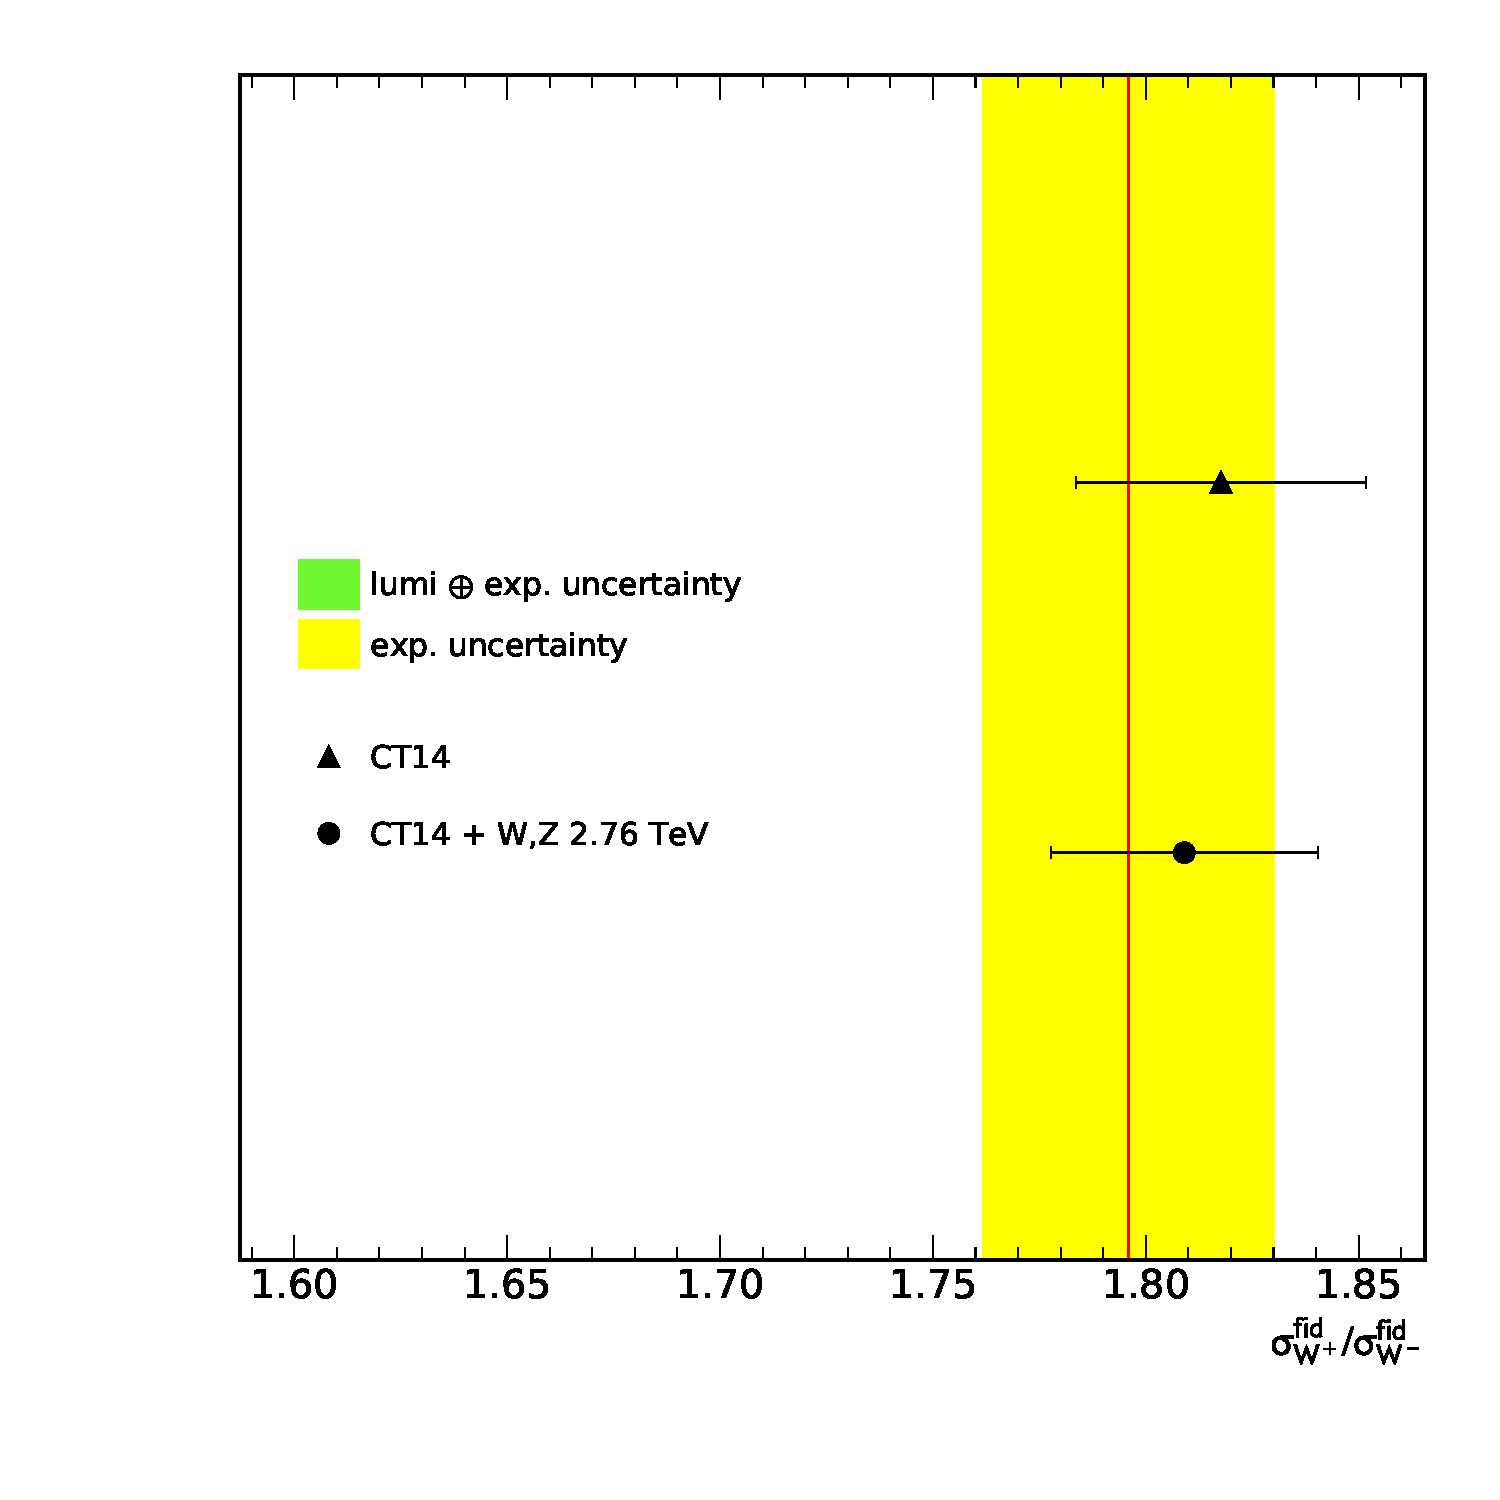
\includegraphics[width=1\textwidth]{Results/PDFImpRatioWpWm.pdf} \\ b)}
\end{minipage}
\caption{The measured a) $W$  and  b) ratio of $W^+$ to $W^-$ fiducial cross sections in combined channel compared to NLO predictions based on the original and profiled CT14 PDF set. }
\label{fig:PDFEffectRatio}
\end{figure}
